\documentclass{article}
\usepackage[skip=5pt plus1pt, indent=0pt]{parskip}
\usepackage[a4paper, total={6in, 8in}]{geometry}
\usepackage{graphicx}
\usepackage{float}
\usepackage{multirow}
\usepackage[table,xcdraw]{xcolor}
\usepackage{booktabs}
\usepackage{amsmath}
\usepackage{multicol}



\title{Notes on Hardware Architectures for Artificial Intelligence}
\date{2023/25/02}
\author{Mattia Morabito}


\begin{document}

  \maketitle
  \pagenumbering{gobble}

  \newpage

  \begin{frame}{\contentsname}
    \begin{multicols}{2}
    \tableofcontents
    \end{multicols}
    \end{frame}
  \newpage

  \pagenumbering{arabic}

  \section{License}
    Copyright © 2023 Mattia Morabito


    Permission is hereby granted, free of charge, to any person obtaining a copy of this document and associated documentation files (the “Document”),
    to deal in the Document without restriction, including without limitation the rights to use, copy, modify, merge, publish, distribute, sublicense,
    and/or sell copies of the Document, and to permit persons to whom the Document is furnished to do so, subject to the following conditions:
    
    The above copyright notice and this permission notice shall be included in all copies or substantial portions of the Document.
    
    THE DOCUMENT IS PROVIDED “AS IS”, WITHOUT WARRANTY OF ANY KIND, EXPRESS OR IMPLIED, INCLUDING BUT NOT LIMITED TO THE WARRANTIES OF MERCHANTABILITY, FITNESS FOR A PARTICULAR PURPOSE AND NON INFRINGEMENT. 
    IN NO EVENT SHALL THE AUTHORS OR COPYRIGHT HOLDERS BE LIABLE FOR ANY CLAIM, DAMAGES OR OTHER LIABILITY, WHETHER IN AN ACTION OF CONTRACT, TORT OR OTHERWISE, ARISING FROM, OUT OF OR IN CONNECTION WITH
    THE DOCUMENT OR THE USE OR OTHER DEALINGS IN THE DOCUMENT.

  \newpage
  
  \section{Introduction}
    Before beginning any discussion on the topics of the course it’s better to keep 
    in mind the definition of Artificial Intelligence to which we will refer during the duration of the course:

    \emph{Artificial Intelligence is the area of computer science that studies the development of hardware and 
    software systems endowed with abilities typical of human beings. Such systems are able to autonomously pursue 
    a given purpose by making decisions that, until then, were usually made by human beings.}

    In particular by hardware and software systems we intend to describe a particular stack composed by:
    \begin{itemize}
      \item \textbf{AI Software (Application)}: The AI-based application running into the IT system
      \item \textbf{AI Software (Framework/Platform/Tool)}: Programs and libraries to control the physical resources and provide tools to build applications (i.e. TensorFlow)
      \item \textbf{AI Hardware}: Hardware to support AI, either specialized or general purpose
    \end{itemize}

    \subsection{AI Hardware classification}
      In the realm of AI Hardware we can list everything from full-on datacenters to tiny IoT nodes. This broad classification while helping us understand the
      reach AI in our modern day does not help as designers. How our application should run? Should it be optimized for data centers? What are the
      advantages and disadvantages of each approach?

      \begin{figure}[H]
        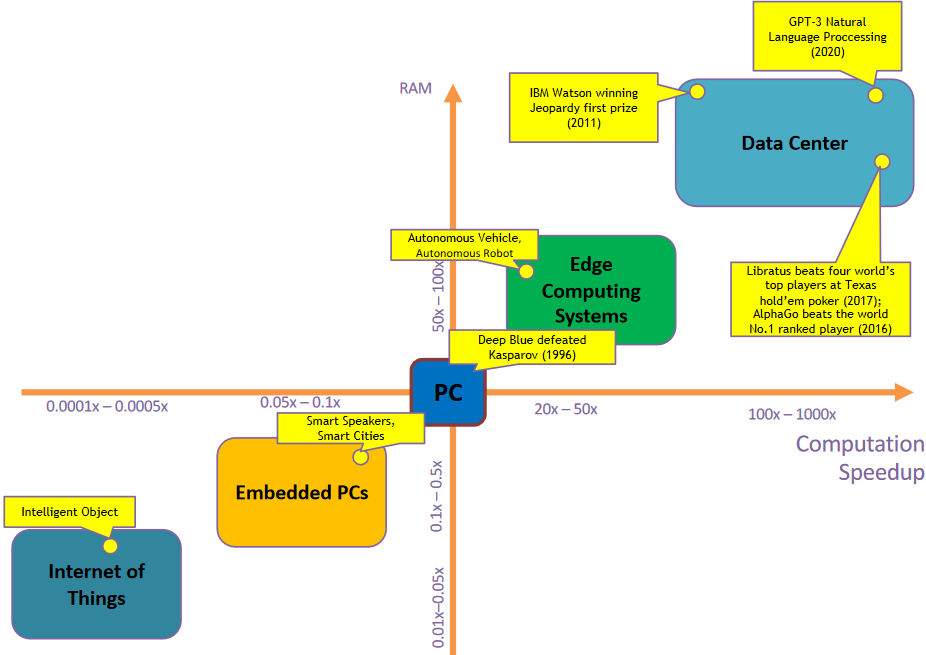
\includegraphics[scale=0.3]{../Images/HWforAI.png}
        \centering
        \caption{AI Hardware classification}
      \end{figure}

      Let's split the spectrum in 4 main sections:

      \subsubsection{Data Centers}
      The datacenter is the perfect environment to run scalable and heavy applications due to the basically infinite amount of processing and storage resources. In this way we can implement
      high performance models while lowering our IT cost and maximizing data reliability, however everything comes at a cost, in particular we require a constant, stable and high speed network connection.
      Moreover, we should particularly focus on security and privacy due to possible attacks while considering a very high power consumption due to constant transmission of data.

      Datacenters are also not able to fit the requirements of time-critical applications such as autonomous driving due to unpredictable latency of the transmission. This single drawback rules them out
      of consideration and poses a need for more responsive and predictable systems in terms of latency.

      \subsubsection{Edge nodes}
      Due to the previous flaws we must move the computation from the cloud to the real world. A fist approach is to move some servers near to the application as is the case for high-speed networking (5G).
      This approach is commonly referred as \emph{Edge Computing} where some Edge nodes are directly integrated in the field. This approach brings high computational capacity, reduced latency for time-critical
      applications and increases the security of the system (decoupling networks and users).

      However, edge nodes are still powerful machines and require a constant power connection while also being connected to cloud.

      \paragraph{The term \emph{Edge} is usually in reference to the computational activity, while for networking we use the term \emph{Fog}}

      \subsubsection{Embedded computers}
      Embedded PC go a step further, they reduce performance while still providing a pretty competent machine while allowing to be distributed in the environment. One of the advantages is the availability of many
      development board which are ready to be programmed while also providing a standard OS interface which hugely simplify the development of the application.

      Still they can be pretty demanding in terms of power, so they need a power connection, and require some hardware design.

      \subsubsection{IoT devices}
      IoT devices are the most integrated and distributed components of the infrastructure. In fact by transition from microprocessors to microcontroller we can hugely reduce their power consumption ($\simeq mW$)
      allowing them to be battery powered. Cost also goes down while still allowing to allocate sensors and actuators to gather data and interact with the environment.

      The processing power is greatly reduced, posing the need for more involved software (i.e.\ lack of OS interface) and hardware design (i.e.\ tight memory and energy requirements)
      to get the most out of each device. By forgoing the cabled connection we also introduce additional challenges related to wireless connectivity (synchronization, networking).

      We should also clarify that there is a difference between a \emph{Connected object}, which is able to connect to the network and exchange data, and a \emph{Smart Object} which is also connected but is also able to
      make decisions based on the information that it gathers.
  
  \subsection{Objectives}
    Our objective is to \emph{move (intelligent) processing as close as possible to data generation units}. This brings a lot of advantages such as:
    \begin{itemize}
      \item \textbf{Increasing autonomy}: by introducing more smart objects which do not rely on other systems
      \item \textbf{Reducing decision-making latency}: fewer unpredictable latencies
      \item \textbf{Reducing transmission bandwidth}: fewer cloud-node communication
      \item \textbf{Increasing energy-efficiency}: since computing is $\simeq 10x$ more efficient than transmitting
      \item \textbf{Increasing Security and Privacy}: local data is processed on the spot and not shared with the whole network
      \item \textbf{Incremental/Adaptive Learning}: environment impervious systems to correctly scale performance
      \item \textbf{Exploiting the ecosystem of units}:
    \end{itemize}

    This however poses some rather interesting challenges due to:
    \begin{itemize}
      \item \textbf{Hardware constraints}: which includes low computational ability, energy and memory
      \item \textbf{Complexity in design and development}: due to the lack of OS interfaces
      \item \textbf{Strong connection between HW, SW and ML}: poising the problem of tight integration
    \end{itemize}
  
  \newpage
  
  \section{Embedded and Edge Hardware}
    Embedded and edge hardware is a very diverse and heterogeneous landscape, however we should find some common architecture to better analyze our requirements
    and our possible solutions. First let's clarify that for \emph{Embedded systems} we mean computers that are designed to perform one specific task (Not general purpose).

    In particular \emph{Embedded system} are meant to run a specific software referred as \emph{Embedded software}.
    \begin{figure}[H]
      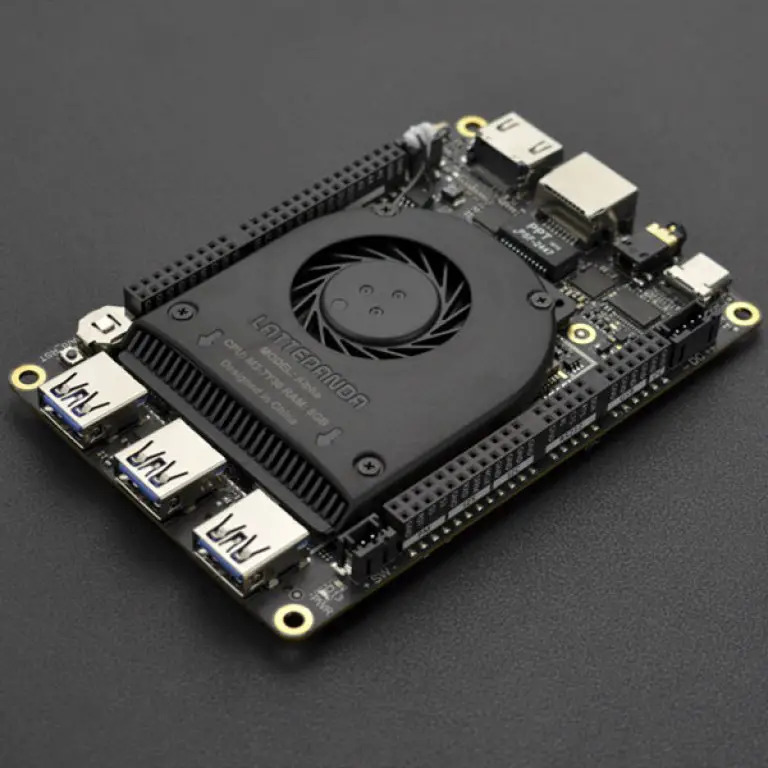
\includegraphics[scale=0.2]{../Images/Lattepanda.jpg}
      \centering
      \caption{Lattepanda SBC (Single Board Computer)}
    \end{figure}

    \subsection{Architecture}
      A generic \emph{Edge device} or \emph{Embedded system} will have the following architecture, as described in the following figure:
      \begin{figure}[H]
        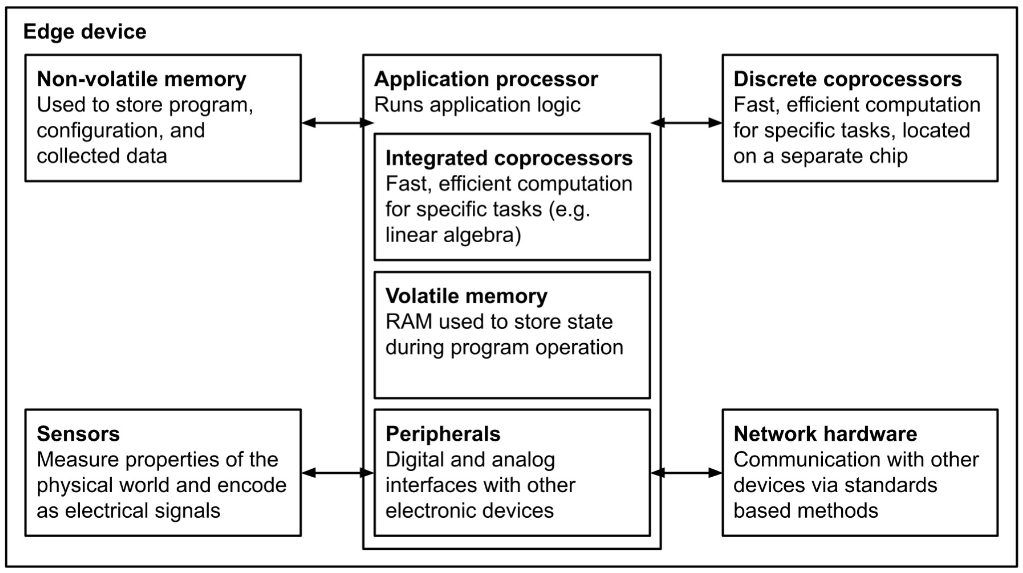
\includegraphics[scale=0.4]{../Images/EdgeArch.PNG}
        \centering
        \caption{Architecture of an edge device}
      \end{figure}

      \subsubsection{Application processor}
        The application processor is a General Purpose Processor (GPP) that coordinates the application and runs most (if not all) the algorithms and logic that make up its program.
        This class of processor in many cases comes pre-equipped with \emph{integrated coprocessor} (or tightly coupled accelerators), built-in hardware to efficiently perform some
        specific computation (Cryptographic algorithms, Floating point arithmetic, DSP etc.).

        In the same package the GPP integrates \emph{Volatile memory} used as working memory during the program execution, however this does not preclude the system from having additional
        memory outside the package. RAM is usually the bottleneck for Edge devices due to the high area and power requirements. Peripherals are also bundled in the same package to enable communication between external electronics devices and the processor.

      \subsubsection{Non-Volatile memory}
        Non-volatile memory are storage devices which are able to maintain data after power off. This is crucial to retain information such as software programs, user
        configuration, and machine learning models. It’s slow to read and extremely slow to write. Even if in the diagram this component is displayed as off-chip in practice some 
        small amount of EEPROM or NAND-Flash can be implemented directly in the GPP chip.

        This kind of memory is absolutely necessary if we think that some application may require our system to be powered on only for a few second every hour (Sampling of some sensors every hour).

      \subsubsection{Discrete coprocessors}
        Discrete coprocessor are basically the same as integrated coprocessor but are located off-chip. This allows for much more complex systems where the coprocessor may be
        even more powerful (and power hungry) than the application processor (i.e. Ultra-Low-Power SoC with a GPU).

      \subsubsection{Sensors}
        Sensors are the interface that our electronic system has with the world, allowing him to gather measurements from the environment and/or from humans. Sensor can be \emph{physical}, as in the measure some physical quantity, or they can be \emph{virtual}, measuring some implicit quantity such as
        transmission speed of a communication channel.

        As output, we get streams of data which are provided in different data formats.

    \subsection{Data storage}
      Now that we understand how our system is composed we should investigate how to gather and store data for our application. In particular each data value can be stored as data structure, such as \emph{Boolean}, \emph{n-bit integers (or Fixed-Point)} or as \emph{n-bit Floating point}.
      
      \begin{quote}
        Storing data as a floating point may be convenient but keep in mind that an operation usually requires $\simeq 10\div 20$ times more energy than the Fixed-Point counterpart
      \end{quote}

      Various sensors also organize data differently such as:
      \subsubsection{Time Series}
        A time series is a sequence of data points indexed in chronological order, at a fixed sampling rate or period (equally spaced). The memory requirement can be computed knowing the sampling period $T_s$ and the number of bits $n$ used for the representation as:

        \begin{equation} 
          N [bits] = \frac{T}{T_s} *n
        \end{equation}

        Where $T$ is the amount of time for which we sample data
      \subsubsection{Audio}
        A special case of time series data, audio signals represent the oscillation of sound waves as they travel through the air. The \emph{Sampling frequency} $f_s [Hz]$, \emph{Quantization or bits per sample} $n [bits]$, \emph{length of the signal} $T [s]$ and \emph{number of channels} $C$ (e.g., mono or stereo) are key aspects.
        Once all the parameters are known we can compute the memory requirement as:
        
        \begin{equation} 
          N [bits] = T*f_s*C*n
        \end{equation}
      
      \subsubsection{Images}
        Images are data that represent the measurements taken by a sensor that captures an entire scene. They have two or more dimensions. In their typical form, they can be thought of as a
        grid of “pixels”, where the value of each pixel represents some property of the scene at the corresponding point in space (stored in $n$ bits). Assuming an image has dimension $W\times K$ with $C$ channels we can compute the memory requirements as:

        \begin{equation} 
          N [bits] = W*K*C*n
        \end{equation}

      \subsubsection{Videos}
        A sequence of (fixed) images reproduced with a suitably high frame rate
        Similarly to image we have $W, K, n$ and $C$ (channels). In addition, we have a \emph{frame rate} $F_r [frames/s]$ and the \emph{length of the video} $T [s]$.
        Once all the parameters are known we can compute the memory requirement as:

        \begin{equation} 
          N [bits] = T*F_r*W*K*C*n
        \end{equation}

        \begin{quote}
          This computation is valid for \emph{raw or uncompressed} video
        \end{quote}

    \subsection{Sensors}
        To give a more complete picture of the embedded hardware we will now list some of the most relevant families of sensor on the market

        \subsubsection{Acoustic and vibration}
          Acoustic and vibration sensor allow us to detect the effects of movement, vibration, and
          human and animal communication at a distance by measuring the effect of vibrations travelling through a
          medium like air (microphones), water (hydrophones) or ground (geophones and seismometers).

          This family of sensors generally produce an audio data describing the variation of pressure in the medium. This information is distributed across frequencies,
          making the sampling rate (or frequency) the most important parameter (Nyquist).
        
        \subsubsection{Visual and scene}
          Camera allow us to acquire the scene information without contact. They can range from tiny and low-power to high quality multi-megapixel sensor     
          They are generally characterized based on \emph{Color channels}, \emph{spectral response} (IR, X-RAY), \emph{pixel size} (sensitivity), \emph{resolution} and \emph{frame rate}.
          Their output is an image (2D/3D) or a video.
        \subsubsection{Motion and position} %maybe use a list
          Motion and position sensors allow us to obtain the spatial information of a target such as position, velocity or acceleration. They come in many types and configurations but the most prominent are: 
          \begin{itemize}
            \item \textbf{Tilt sensors}: which measure orientation by a mechanical switch.
            \item \textbf{Accelerometers}
            \item \textbf{Gyroscopes}: which measure the rate of rotation;
            \item \textbf{Time of flight (ToF)}: which measure the distance of the target object from the sensor by electromagnetic emissions.
            \item \textbf{Real time locating systems}: multiple transceivers in fixed locations around a building to track the position of individual objects.
            \item \textbf{GPS}: which use satellites to determine the location of a device.
          \end{itemize}
          Their measurements are usually represented as time series.

        \subsubsection{Force and tactile}
          Helpful in facilitating user interaction, understanding the flow of liquids and gases, or
          measuring the mechanical strain on an object:
          \begin{itemize}
            \item \textbf{Buttons and switches}: provide a binary signal.
            \item \textbf{Capacitative touch sensors}: measure the amount that a surface is being touched by a conductive object, like a human finger.
            \item \textbf{Strain gauges}: measure how much an object is being deformed.
            \item \textbf{Load cells}: these measure the amount of physical load that is applied.
            \item \textbf{Flow sensors}: measure the rate of flow in liquids and gases.
            \item \textbf{Pressure sensors}: used to measure pressure of a gas or liquid, either environmental or inside a system (e.g., inside a car tire).
          \end{itemize}
          Measurements are typically represented as a time series.
        \subsubsection{Optical, electromagnetic and radiation}
          Sensors measuring electromagnetic radiation, magnetic fields as well as current and voltage:
          \begin{itemize}
            \item \textbf{Photosensors}: detect light at various wavelengths, both visible and invisible to the human eye.
            \item \textbf{Color sensor}: photosensors to measure the precise color of a surface, helpful for recognizing different types of objects.
            \item \textbf{Spectroscopy sensors}: measure the way that various wavelengths of light are absorbed and reflected by materials, giving an edge AI system insight into their composition.
            \item \textbf{Magnetometer}: measure the strength and direction of magnetic fields (a digital compass).
            \item \textbf{Inductive proximity sensors}: electromagnetic field to detect nearby metal (detect vehicles for traffic monitoring).
            \item \textbf{Electromagnetic field (EMF) meters}: measure the strength of electromagnetic fields (e.g., emitted by industrial equipment).
            \item \textbf{Current and voltage sensor}
          \end{itemize}
          Measurements are typically represented as a time series.
        \subsubsection{Environmental and chemical}
          Sensors measuring physical quantities related to the environment in which the device is in. The more common one include:
          \begin{itemize}
            \item \textbf{Temperature sensors}
            \item \textbf{Gas sensors}: e.g., humidity or carbon dioxide sensors.
            \item \textbf{Particulate matter sensor}: monitor pollution levels.
            \item \textbf{Biosignals sensors}: e.g., measurement of electrical activity in the human heart (electrocardiography) and brain (electroencephalography).
            \item \textbf{Chemical sensors}: measure the presence or concentration of specific chemicals.
          \end{itemize}
          Measurements are typically represented as a time series

    \newpage

    \subsection{Our choice}
      In this course we are going to deal mostly with Microcontrollers which will represent the basic technological block of our pervasive
      applications. Their size, generally low cost the fact that every useful component is already embedded in the same piece of silicon makes them the perfect choice.

      However, we must also take into consideration that there is no operating system on this platform, so the \emph(firmware) is directly executed on the hardware and 
      includes the low-level instructions to connect the peripherals. The programming language can either be high-level (C, C++) or low-level (platform specific Assembly).

      Other platform like SoC are present in the embedded AI landscape but for out purpose the higher computing power is not worth the low energy efficiency (w.r.t. MCUs) and the larger cost.
      By keeping in mind the data storage and computation requirements we can now compile a summary table representing the capabilities of each platform.

      \begin{table}[H]
      \resizebox{\columnwidth}{!}{%
      \begin{tabular}{|cc|cccccc|}
        \hline
        \multicolumn{2}{|c|}{}                                                   & \multicolumn{2}{c|}{Time-Series}                                         & \multicolumn{1}{c|}{}                        & \multicolumn{2}{c|}{Images}                                                &                          \\ \cline{3-4} \cline{6-7}
        \multicolumn{2}{|c|}{\multirow{-2}{*}{Device vs Data}}                   & \multicolumn{1}{c|}{Low-frequency} & \multicolumn{1}{c|}{High-frequency} & \multicolumn{1}{c|}{\multirow{-2}{*}{Audio}} & \multicolumn{1}{c|}{Low resolution} & \multicolumn{1}{c|}{High resolution} & \multirow{-2}{*}{Video}  \\ \hline
        \multicolumn{1}{|c|}{}                      & Low-end                    & \cellcolor[HTML]{F8FF00}           & \cellcolor[HTML]{F8FF00}            & \cellcolor[HTML]{FE0000}                     & \cellcolor[HTML]{FE0000}            & \cellcolor[HTML]{FE0000}             & \cellcolor[HTML]{FE0000} \\ \cline{2-2}
        \multicolumn{1}{|c|}{}                      & High-end                   & \cellcolor[HTML]{34FF34}           & \cellcolor[HTML]{34FF34}            & \cellcolor[HTML]{34FF34}                     & \cellcolor[HTML]{34FF34}            & \cellcolor[HTML]{F8FF00}             & \cellcolor[HTML]{F8FF00} \\ \cline{2-2}
        \multicolumn{1}{|c|}{\multirow{-3}{*}{MCU}} & High-end with accelerator  & \cellcolor[HTML]{34FF34}           & \cellcolor[HTML]{34FF34}            & \cellcolor[HTML]{34FF34}                     & \cellcolor[HTML]{34FF34}            & \cellcolor[HTML]{34FF34}             & \cellcolor[HTML]{F8FF00} \\ \cline{1-2}
        \multicolumn{1}{|c|}{}                      & Vanilla                    & \cellcolor[HTML]{34FF34}           & \cellcolor[HTML]{34FF34}            & \cellcolor[HTML]{34FF34}                     & \cellcolor[HTML]{34FF34}            & \cellcolor[HTML]{34FF34}             & \cellcolor[HTML]{34FF34} \\ \cline{2-2}
        \multicolumn{1}{|c|}{\multirow{-2}{*}{SoC}} & With accelerator           & \cellcolor[HTML]{34FF34}           & \cellcolor[HTML]{34FF34}            & \cellcolor[HTML]{34FF34}                     & \cellcolor[HTML]{34FF34}            & \cellcolor[HTML]{34FF34}             & \cellcolor[HTML]{34FF34} \\ \cline{1-2}
        \multicolumn{2}{|c|}{Edge Server}                                        & \cellcolor[HTML]{34FF34}           & \cellcolor[HTML]{34FF34}            & \cellcolor[HTML]{34FF34}                     & \cellcolor[HTML]{34FF34}            & \cellcolor[HTML]{34FF34}             & \cellcolor[HTML]{34FF34} \\ \cline{1-2}
        \multicolumn{2}{|c|}{Cloud}                                              & \cellcolor[HTML]{34FF34}           & \cellcolor[HTML]{34FF34}            & \cellcolor[HTML]{34FF34}                     & \cellcolor[HTML]{34FF34}            & \cellcolor[HTML]{34FF34}             & \cellcolor[HTML]{34FF34} \\ \hline
      \end{tabular}%
      }
      \caption{Summary of platform capabilities}
      \end{table}

  \newpage

  \section{Algorithms for Embedded and Edge AI}
    Now that we have a clear view of the hardware architecture for our system we can begin discussing the AI Application that it will be running
    The software can now be segmented in 3 main components as shown in figure: 

    \begin{figure}[H]
      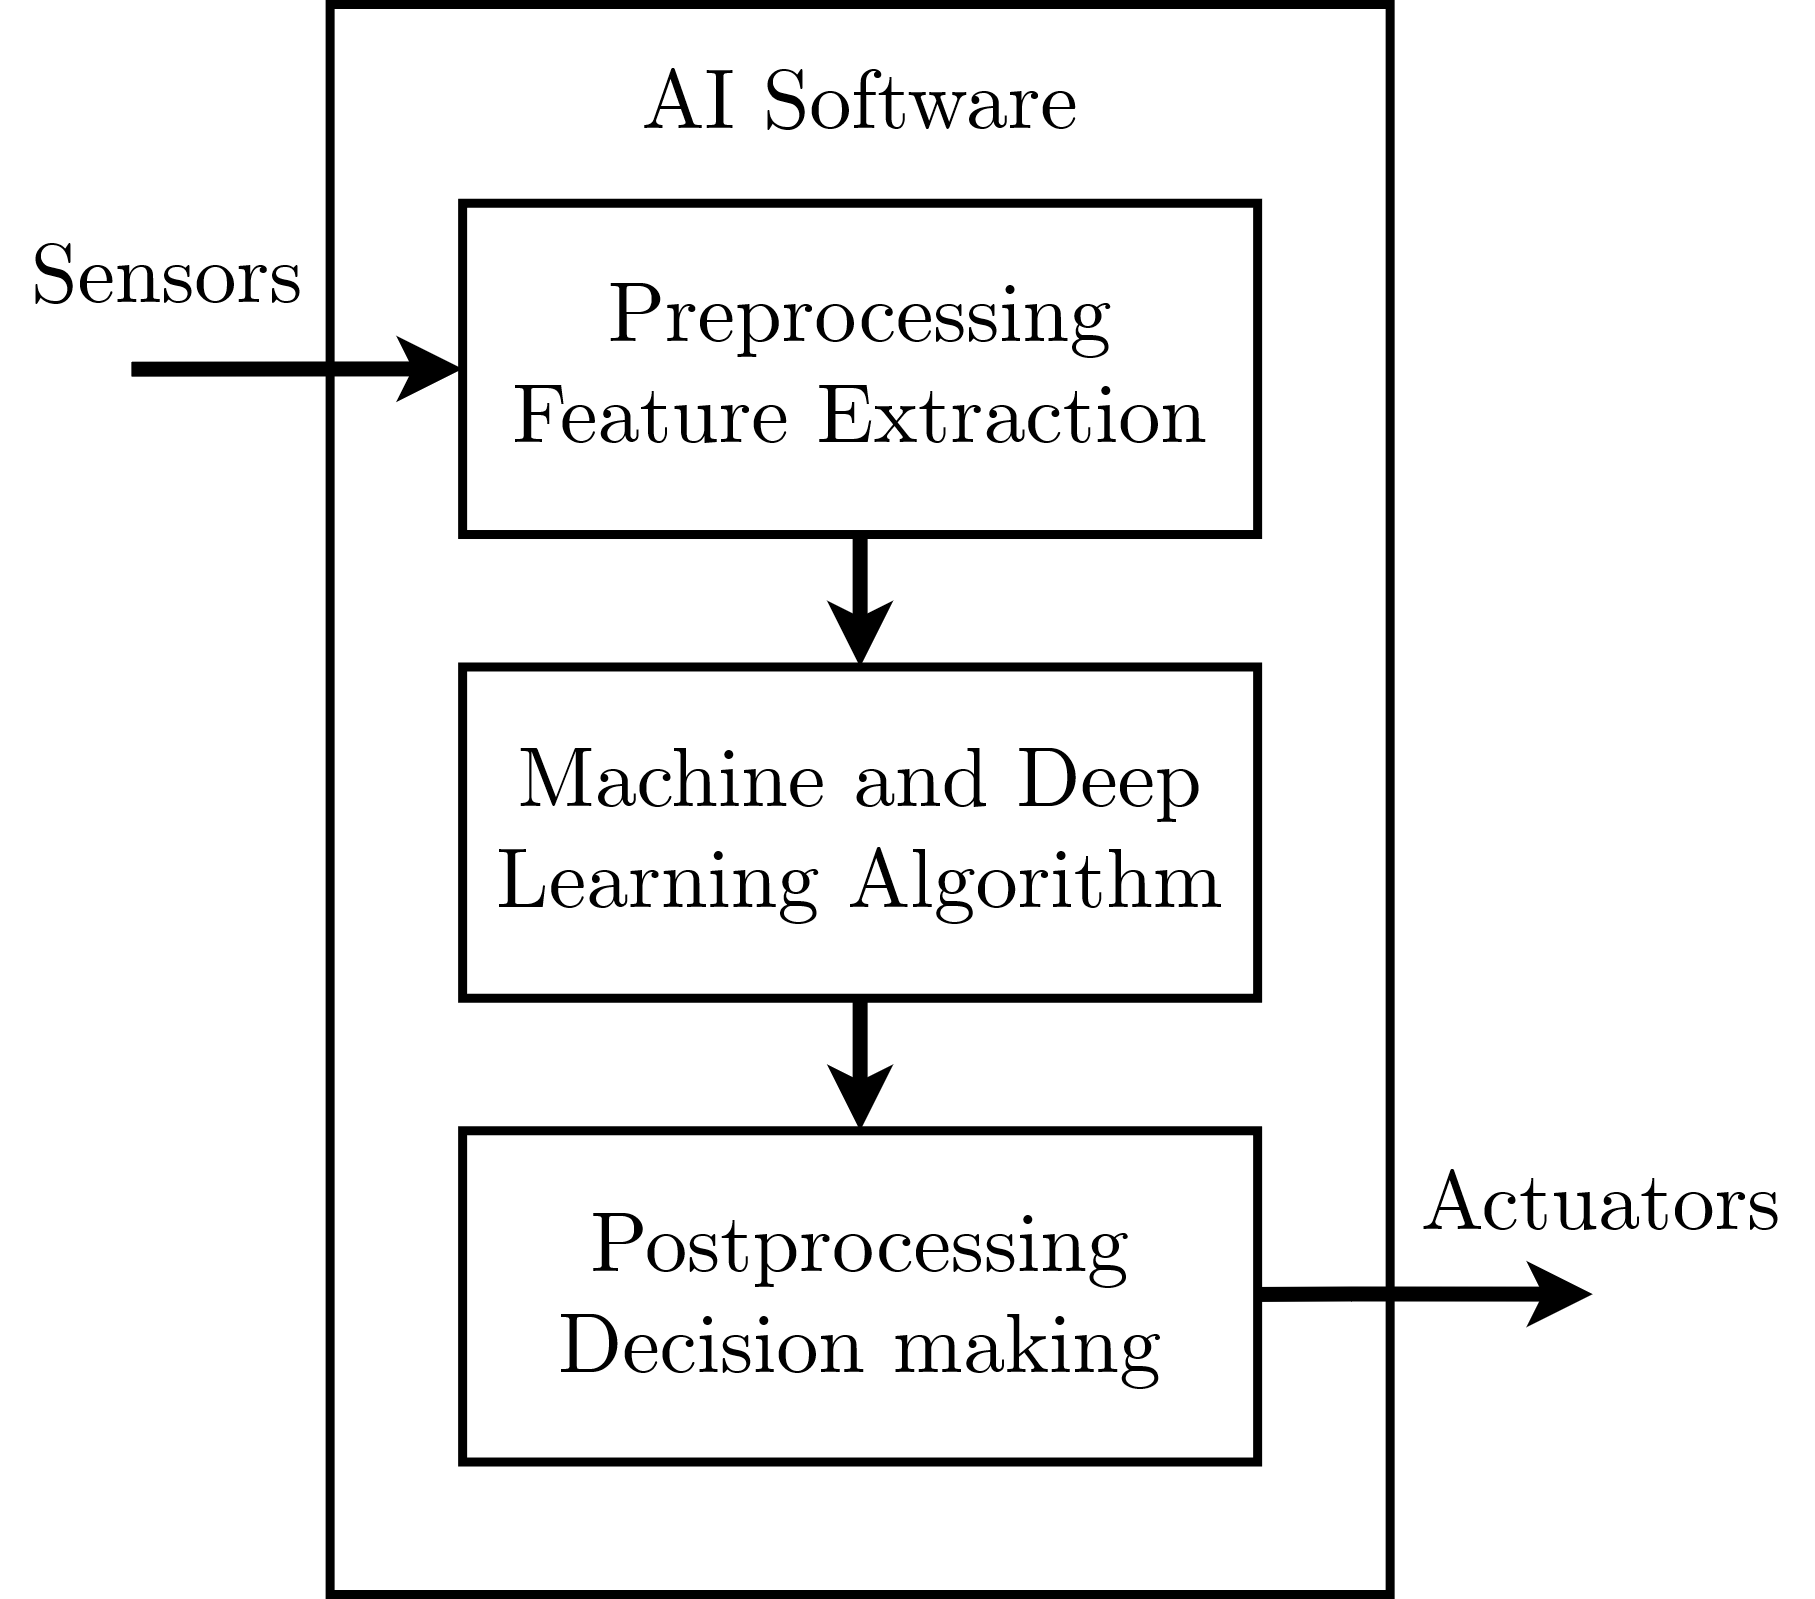
\includegraphics[scale=0.15]{../Images/AI_software.png}
      \centering
      \caption{AI Software stack}
    \end{figure}

    \subsection{Preprocessing \& Feature Extraction}
      The output of our sensor is a raw and noisy data stream which must be processed before entering our Machine/Deep Learning Model. This goal can be achieved by 3 main methodologies.
      \subsubsection{Data segmentation}
        The stream of data coming into our system is continuous however the model can only work on a finite set of data, for this reason we must find a method to correctly segment our stream into blocks
        which will then be used as input in the algorithm. The length of this data block is defined by us and must take into consideration the type of data, the \emph{latency} of the algorithm and the memory constraints.

        This before mentioned \emph{latency} defines how fast our system can process a chunk of data. While this constraint is usually neglected in cloud application, were the inference time is always negligible or not of interest, in embedded systems which follow the
        \emph{always on Machine Learning} approach is a key parameter. A simple example can be made considering autonomous driving vehicles, where the algorithm governing the steering and braking must be able to react in fractions of second to avoid accidents. The design choice 
        of the algorithm has a strong effect on the computational requirement (the latency) as well as the memory demand.

        So by expanding our data chunk we increase the amount of information reaching our model, in turn increasing the accuracy, but both our memory requirements and latency increase which may or may not be acceptable depending on the application.

        Even if we decouple data acquisition and processing latency will still set our system maximum \emph{inference rate} (the rate at which the system is able to acquire and process the data). The limited inference rate also creates the problem of data loss, while our system is processing we can't store an infinite amount of data, and some
        of the chunk that we discard are bound to have relevant information in them. This issue can be slightly mitigated if we overlap the data chunks, however while this decrease the risk of losing information it requires lower latency to make it work correctly and renders our observation non i.i.d (independent identically distributed).
        \begin{figure}[H]
          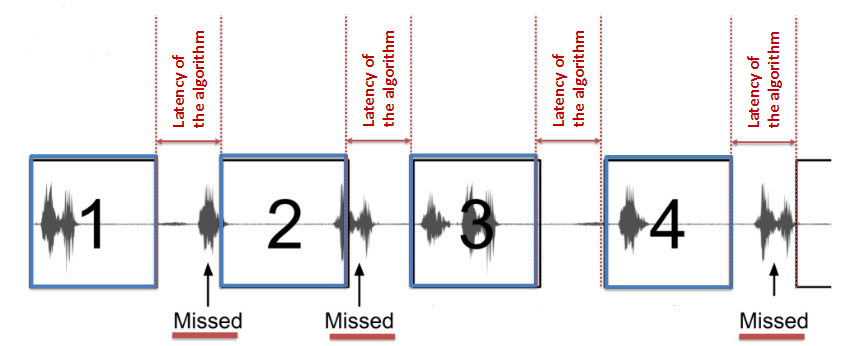
\includegraphics[scale=0.55]{../Images/Missing_data.png}
          \centering
          \caption{Example of missed data due to latency}
        \end{figure}

        \begin{figure}[H]
          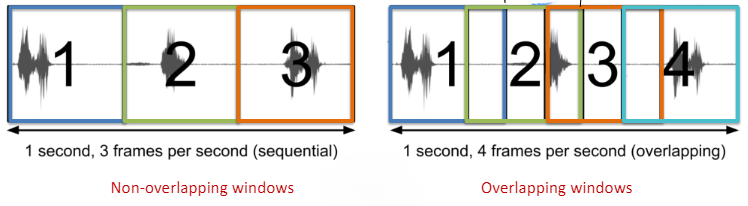
\includegraphics[scale=0.6]{../Images/Chunk_overlap.png}
          \centering
          \caption{Chunk Overlapping}
        \end{figure}
      \subsubsection{Digital processing algorithms for data preprocessing}
        Once our chunks are defined we can apply digital signal processing algorithms to remove noise and highlight
        relevant portions of the signal.

        As a first step if some data points are missing we want to reconstruct them by either:
        \begin{itemize}
          \item \textbf{Global filling methods}: in which we use the whole chunk to fill the missing observations.
          \item \textbf{Local filling methods}: in which we use neighboring data to fill the missing observation (only applicable in situation where for each data point we should make a decision).
          \item \textbf{Deletion}: in which we choose not to use time periods that have missing data at all.
        \end{itemize}

        Also, we might have situations in which time series have different sampling frequencies. This is a problem for our model and is fixable by either:
        \begin{itemize}
          \item \textbf{Upsampling}: increasing the sampling frequency artificially by adding data points in between observations (replication, interpolation). We must be aware that while this is a
          viable method we increase the memory footprint while not adding any relevant information.
          \item \textbf{Downsampling}: decreasing the sampling frequency artificially by only saving a data point every N (subsampling). In this method while we are losing significant information we are also reducing the memory footprint.
        \end{itemize}
        In general, we normalize to the slowest sample while minding the aliasing. This is also applicable to spacial information such as images but instead of frequency we deal with spacial resolution either by keeping the shape of the data (downsampling, interpolation) or by modifying it (cropping, resizing).
        It is particularly useful since usually the maximum input size of the model is a constraint given by memory limitation (model, data size).

        Last but not least the data may need to filtered to only consider information relevant to the application. This is quite convenient since many embedded and processor support fast and energy-efficient computation of filtering operations (LP, HP, BP).
    
      \subsubsection{Feature Extraction}
        Extracting the relevant features in some data is a challenging task and usually requires the help from a field expert however there are some basic analysis techniques that we can employ such as:
        \begin{table}[H]
          \centering
          \begin{tabular}{ccc}
            \hline
            \multicolumn{3}{c}{Domain}                                          \\ \hline
            \multicolumn{2}{c|}{Time}                       & Frequency         \\ \hline
            Mean          & \multicolumn{1}{c|}{SNR}        & Variance of peaks \\
            PCA           & \multicolumn{1}{c|}{Peak Decay} & Max amplitude     \\
            Max amplitude & \multicolumn{1}{c|}{Energy}     & Main frequencies  \\ \hline
            \multicolumn{3}{c}{Spectrogram}                                     \\ \hline
          \end{tabular}
          \caption{Feature extraction basic techniques}
        \end{table}

        Images also have some basics techniques for feature detection, mostly implemented by libraries such as \emph{OpenCV} (for SoC) or \emph{OpenMV} (for MCUs). Some examples are \emph{Edge, Corner, Blob and Ridge} detection.
        
      \subsubsection{Feature combination and data normalization} 
        As a last step me must combine all of our feature together to create the input vector of our model.
        \begin{figure}[H]
          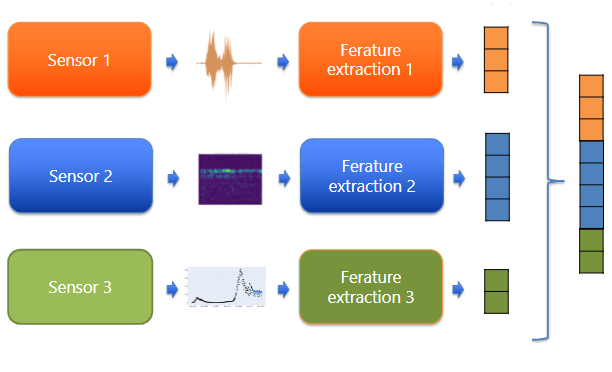
\includegraphics[scale=0.55]{../Images/Feature_combination.png}
          \centering
          \caption{Feature combination example}
        \end{figure}

        While simple consideration have to made in case of features with different scales which may lead to model under/over fitting. This can be avoided by:
        \begin{itemize}
          \item \textbf{Min-Max Normalization}: normalizing the data to have everything in the $[0,1]$ range
          \begin{equation} 
            x_i^{norm} = \frac{x_i- MIN_i(x_i)}{MAX_i(x_i)-MIN_i(x_i)}
          \end{equation}
          \item \textbf{Standardization}: removing mean and dividing by the standard deviation
          \begin{equation} 
            x_i^{std} = \frac{x_i- MEAN(x_i)}{STD(x_i)}
          \end{equation}
        \end{itemize}
        Where all parameter may vary with time and must be correctly tuned to achieve the tightest range to maximize the model performance. 
    \subsection{Machine and Deep Learning Algorithm}
      Our goal now is to apply machine/deep learning algorithms on the preprocessed data to generate and output, however since the listing every algorithm will be impossible it is best to deliver a first order classification
      of algorithms based on their functionality: 
      \begin{table}[H]
        \resizebox{\textwidth}{!}{%
        \begin{tabular}{@{}lll@{}}
          \toprule
          \multicolumn{1}{c}{Functionality} & \multicolumn{2}{c}{Examples}                                                                        \\ \midrule
          Classification                    & Classify micro-acoustic emissions of a rock face     & Recognize bird vocalizations                 \\
          Regression                        & Measure the level of a liquid in cup                 & Estimate the number of people in the room    \\
          Object detection                  & OpenDataCam                                          & Counting the number of attendees to an event \\
          Segmentation                      & Identification of logically coherent regions of data & Street view for autonomous driving           \\
          Anomaly detection                 & Detect persons in a conveyor belt                    & Detect micro-acoustic emissions              \\
          Prediction                        & Predict the next value of a time series              & Weather forecasting                          \\
          Feature reduction                 & \multicolumn{2}{l}{Compress or extract features from audio chunks to reduce the size}               \\ \bottomrule
        \end{tabular}%
        }
        \caption{Algorithm's classification by functionality}
      \end{table}

      Another possible classification can be achieved by considering the implementation, as such we may have:
      \begin{itemize}
        \item \textbf{Conditional logic}: In cases where we can find a deterministic model to carry out the decision we may employ a series of conditional statements to implement the application.
        This is not machine learning however since the system does not learn anything and is inflexible to more general cases. Does not require training and is the most efficient way to implement our application.
        \item \textbf{Machine Learning}: In machine learning before using the model we must rely on a field-specific expert to extract the relevant feature, which then become the input of our model. In other word the machine learning
        model only learns the how to classify based on the features.
        \item \textbf{Deep Learning}: In some situation we may not have the capabilities to extract the relevant features from out data, deep learning solves this issue by allowing the model to carry out this step. While this seems like
        the obvious choice this class of algorithm require much deeper pipelines and is rather data-hungry. Also, by decoupling the feature extraction we have no transparency on the decision policy (i.e. a model may learn to classify an image by the background and not the subject).
      \end{itemize}

      In this course we will focus on implementing machine and deep learning algorithms on IoT and Edge systems, in this context our framework of choice is \emph{TinyML}. It is mandatory to point out that not the whole tool chain is necessarily implemented on the distributed devices.
      Some policy choices regarding this can be found on the following figure:
      \begin{figure}[H]
        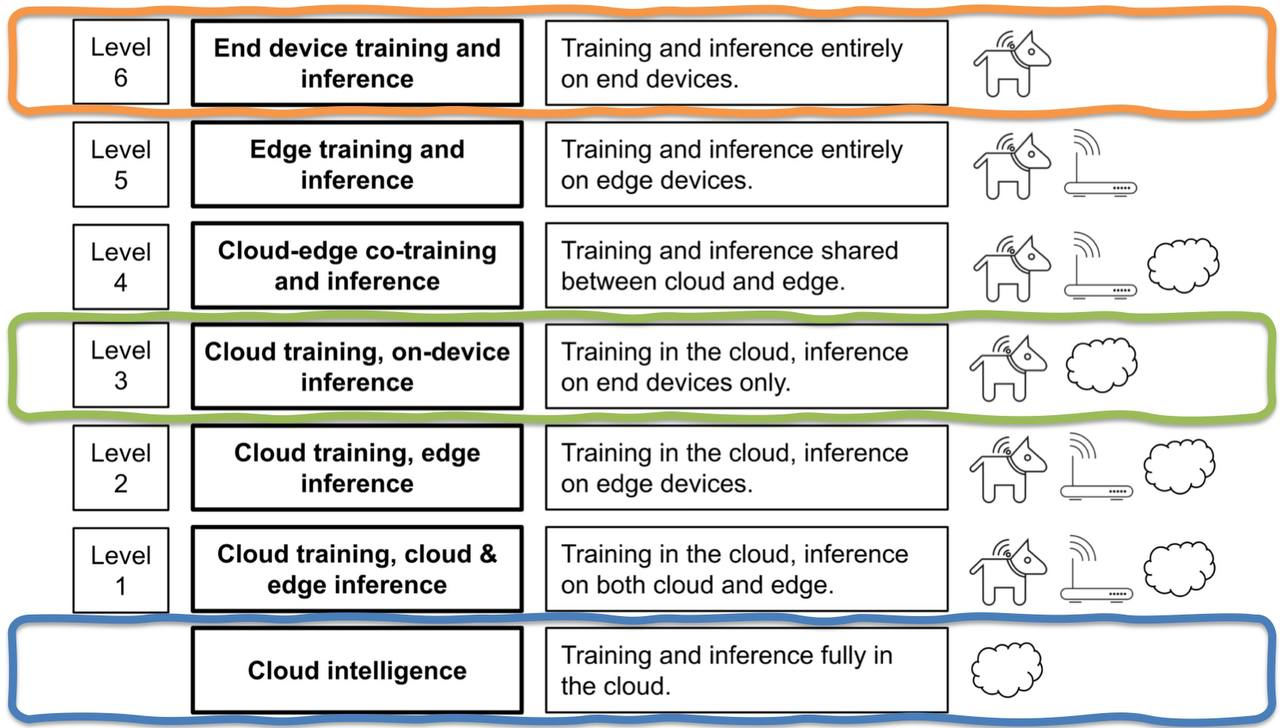
\includegraphics[scale=0.25]{../Images/AITrainingLevels.jpg}
        \centering
        \caption{Levels of integrations concerning AI}
      \end{figure}

    \subsection{Post-processing \& Decision-making}
  
  \newpage
  \section{Basics of Machine learning}
    It is important to review some basics concepts of machine learning to fully understand the future subjects. As such, in general, the goal of learning given a data generating process is to identify
    and build the simplest approximating model able to explain both the past and future instances of the process. 

    To this aim we must identify the possible sources of error (or risk) in our model. An elegant and complete representation of the error sources is:

    \begin{equation} 
      \epsilon = \epsilon_E + \epsilon_A + \epsilon_I
    \end{equation}

    Where the total error is the superposition of:
    \begin{itemize}
      \item $\epsilon_I$ is the error that depends only on the structure of the learning problem and, for this reason, can be reduced only by improving the problem itself (i.e. non-removable noise).
      \item $\epsilon_A$ is the approximation error that depends on how close the model family is to the process generating data (i.e. is the model the correct approximation of the process). In the tinyML space this is the most relevant contribution.
      \item $\epsilon_E$ is the estimation error that depends on the ability of the learning algorithm to select parameters which correctly represent the process. Mainly dependent on the amount of data available.
    \end{itemize}

    We will mostly discuss neural networks since the \emph{Universal approximation theorem} states: 
    \begin{quote}
      A feedforward network with a single hidden layer containing a finite number of neurons approximates any continuous function defined on compact subsets.
    \end{quote}

    Which, while not giving any constructive information about the number of neurons is actually required, allows us to assume that the approximation error will be always $0$. As a consequence we need to worry only about the estimation error.

    But how can we evaluate the performance of our model? Below are listed some common validation techniques such as:
    \begin{itemize}
      \item \emph{Apparent Error Rate (AER), or resubstitution}: The whole set is used both to infer the model and to estimate its error
      \item \emph{Sample Partitioning (SP)}: Training set and Evaluation set are obtained by randomly splitting the whole set in two disjoint subsets. The training set is used to estimate the model and the evaluation set to estimate its accuracy.
      \item \emph{Leaving-One-Out (LOO)}: The evaluation set contains one pattern in the set, and the training set contains the remaining $n - 1$ patterns. The procedure is iterated $n$ times by holding out each pattern in the whole set, and the resulting $n$ estimates are averaged.
      \item \emph{W-fold Crossvalidation (wCV)}: The set is randomly split into $w$ disjoint subsets of equal size. For each subset the remaining $w - 1$ subsets are merged to form the training set and the reserved subset is used as evaluation set. The $w$ estimates are averaged.
    \end{itemize}

  \newpage
  \section{Model requirements}
    We now want to analyze the sources of complexity coming from our model, both in memory and computational terms. To this aim we can use as a case study the convolutional neural network in figure:

    \begin{figure}[H]
      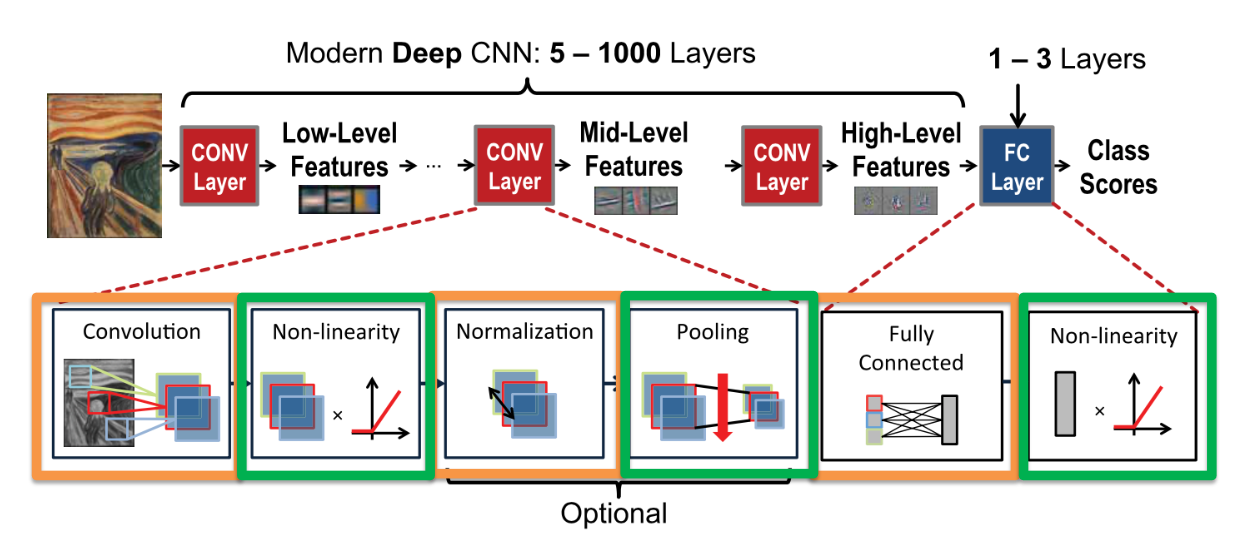
\includegraphics[scale=0.35]{../Images/CNN.png}
      \centering
      \caption{Convolutional Neural Network (CNN)}
    \end{figure}
    
    Where the layers highlighted in orange are processing layers with trainable parameters which need to be trained and stored while the green do not possess trainable parameters. In general, we can split the pipeline in a filtering phase composed of mostly convolutional layers, where we learn which feature to extract from the raw data, 
    and a classification phase composed mainly of dense (or fully connected) layers.

    \subsection{Convolutional layers}
      In generic convolutional layer we have 3 main components to consider, the \emph{Input Feature Map} (a.k.a. the input), the \emph{Filters} and the \emph{Output Feature Map} (a.k.a. the output)
      With the generic dimension showed in figure we can easily compute both the memory (bytes) and computational demand (MACs)
      
      \begin{figure}[H]
        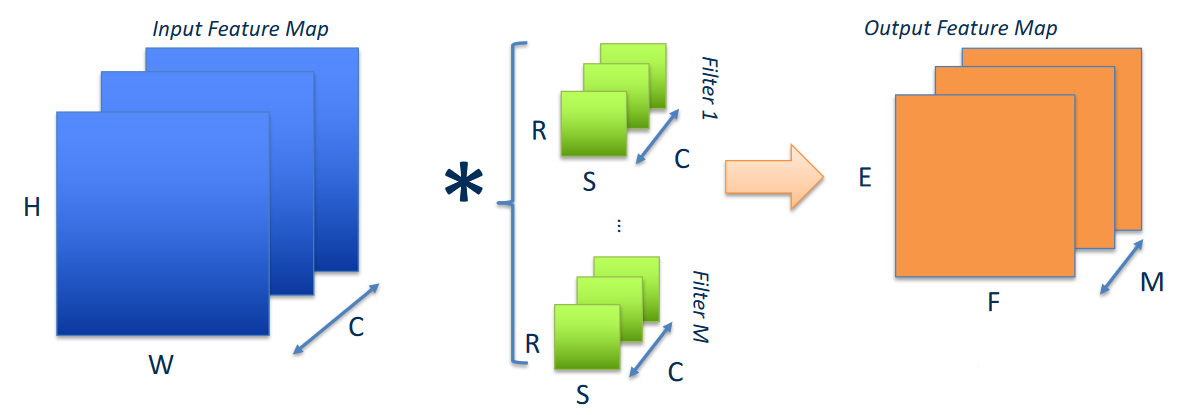
\includegraphics[scale=0.35]{../Images/ConvLayers.png}
        \centering
        \caption{Convolutional layer}
      \end{figure}
      
      Naming $C$ as the number of channels, $M$ as the number of filter, $U$ as the stride and being  $E = (H-R+U)/U$ and $F = (W-R+U)/U$ the output dimension we get the memory requirements as:
      \begin{equation}
        N [bytes] = M \times R \times S \times C + M
      \end{equation}

      While the computational requirements (neglecting the bias) for the inference are:
      \begin{equation}
        N [MACs] = E \times F\times R\times S\times C\times M
      \end{equation}

      We can immediately see how the memory requirements do not depend on the input size while the MAC have an indirect dependence due to the output size.
    \subsection{Dense layers}
    The dense layers are much simpler, given the dimensions shown in figure we can immediately say:
      \begin{figure}[H]
        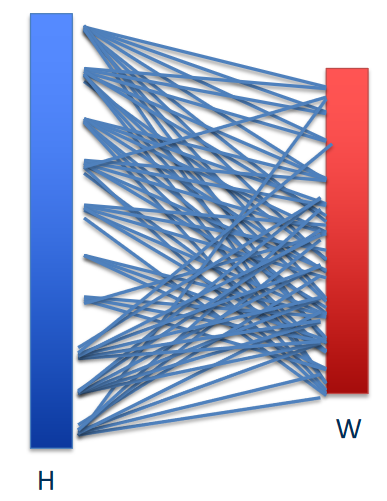
\includegraphics[scale=0.35]{../Images/DenseLayers.png}
        \centering
        \caption{Dense layer}
      \end{figure}

      \begin{equation}
        N [bytes] = H\times W + W
      \end{equation}
      \begin{equation}
        N [MACs] = H\times W
      \end{equation}

    \subsection{Feature maps}
      We must also consider the feature map occupation, considering a generic convolutional layer with the dimension of point 6.1 we would get
      \begin{equation}
        N_C [bytes] = M_i + M_o  = H\times W\times C + E\times F\times M
      \end{equation}
      
      Instead for a dense layer:
      \begin{equation}
        N_D [bytes] = M_i + M_o  = H + W
      \end{equation}

      In reality, we only need to store a maximum of 2 feature maps at a time so by considering the biggest 2 consecutive maps we can reduce this memory occupation.
    \subsection{Considerations}
      In general in a deep learning pipeline the dense layer will pose the greatest memory occupation while the Convolutional layers will amount to most of the computation. This creates an interesting
      trade-off since the amount of convolutional layers is usually directly proportional to the quality of the extracted features while bigger dense layers contribute to a more complex classifier.

  \section{Tiny architectures}
    Nowadays, models keep getting bigger and bigger, this is fundamentally incompatible with our application field, and we must take steps to make models run on IoT devices. In other terms we must rethink our model
    to fit the technological constraints especially since using a smaller architecture does not necessarily mean less accuracy.

    \subsection{Re-design of the CNN architecture}
      The first step must be to make architectural changes to existing network to make them IoT-Friendly while keeping our accuracy. We will explore three popular families of architectures for tiny devices currently employed.
      \subsubsection{SqueezeNet (2016)}
        SqueezeNet architectures were developed to: allow more efficient distributed training (since communication overhead is proportional to model size) due to the popularity of the federated learning approach; to reduce the overhead of exporting new models to the client (faster updates) and to allow
        for feasible FPGA and embedded deployments. As a result we want to identify smaller CNN architectures with equivalent accuracy and to redefine the design space for smaller Neural Networks.

        The author outlines 3 main strategies \cite{SNet}:
        \begin{itemize}
          \item Replace 3$\times$3 filters with 1$\times$1 filters. Given a budget of a certain number of convolution
          filters, we will choose to make the majority of these filters 1$\times$1, since a 1$\times$1 filter has 9X fewer
          parameters than a 3$\times$3 filter.
          \item Decrease the number of input channels to 3$\times$3 filters. Consider a convolution layer
          that is composed entirely of 3$\times$3 filters. The total quantity of parameters in this layer is (number of
          input channels) * (number of filters) * (3*3). So, to maintain a small total number of parameters
          in a CNN, it is important not only to decrease the number of 3$\times$3 filters (see Strategy 1 above), but
          also to decrease the number of input channels to the 3$\times$3 filters.
          \item Downsample late in the network so that convolution layers have large activation
          maps. In a convolutional network, each convolution layer produces an output activation map with
          a spatial resolution that is at least 1$\times$1 and often much larger than 1$\times$1. The height and width of
          these activation maps are controlled by: (1) the size of the input data (e.g. 256$\times$256 images) and (2) 
          the choice of layers in which to downsample in the CNN architecture.
        \end{itemize}

        These 3 strategies are then condensed in the \emph{Fire Module} defined as follows. A Fire module comprises: a squeeze convolution layer
        (which has only 1$\times$1 filters), feeding into an expand layer that has a mix of 1$\times$1 and 3$\times$3 convolution
        filters. The liberal use of 1$\times$1 filters in Fire modules is an application
        of Strategy 1. We expose three tunable dimensions (hyperparameters) in a Fire
        module: $s1x1$, $e1x1$, and $e3x3$. In a Fire module, $s1x1$ is the number of filters in the squeeze layer
        (all 1$\times$1), $e1x1$ is the number of 1$\times$1 filters in the expand layer, and $e3x3$ is the number of 3$\times$3 filters
        in the expand layer. When we use Fire modules we set $s1x1$ to be less than ($e1x1$ + $e3x3$), so the
        squeeze layer helps to limit the number of input channels to the 3$\times$3 filters, as per Strategy 2.

        \begin{figure}[H]
          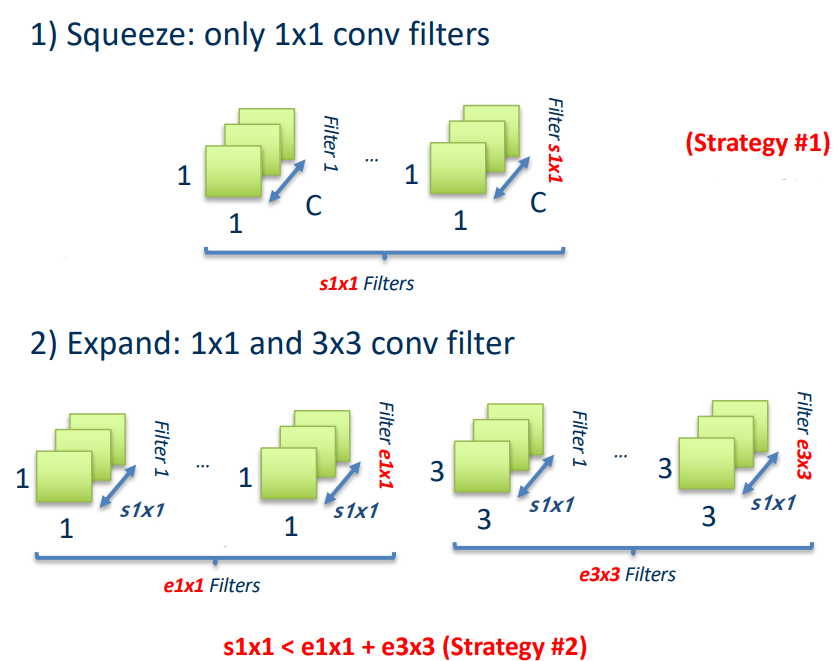
\includegraphics[scale=0.35]{../Images/FireModule.png}
          \centering
          \caption{Fire Module}
        \end{figure}

        Using AlexNet as a case study we can see how this practices can achieve a 510x reduction in size without any accuracy loss, as shown in the next figure:

        \begin{figure}[H]
          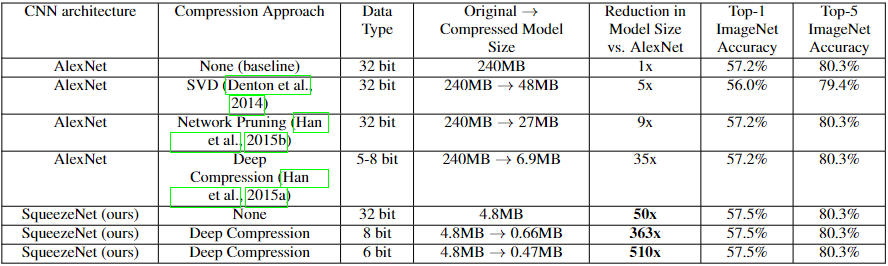
\includegraphics[scale=0.6]{../Images/squeezenettable.png}
          \centering
          \caption{Fire Module}
        \end{figure}

        This particularly important in the framework of sustainability since fewer parameters and less computing time reduces the power needed to run an application.
        Further optimization can be applied by means of simple or complex bypass. Where the \emph{Simple bypass} architecture adds bypass connections around Fire modules 3, 5, 7, and 9,
        requiring these modules to learn a residual function between input and output while the \emph{Complex bypass} adds a bypass that includes a 1$\times$1 convolution layer with the number of
        filters set equal to the number of output channels (Extra parameters to be trained). However, results only support the use of the simple bypass due to the added parameters of the complex one.

        \begin{figure}[H]
          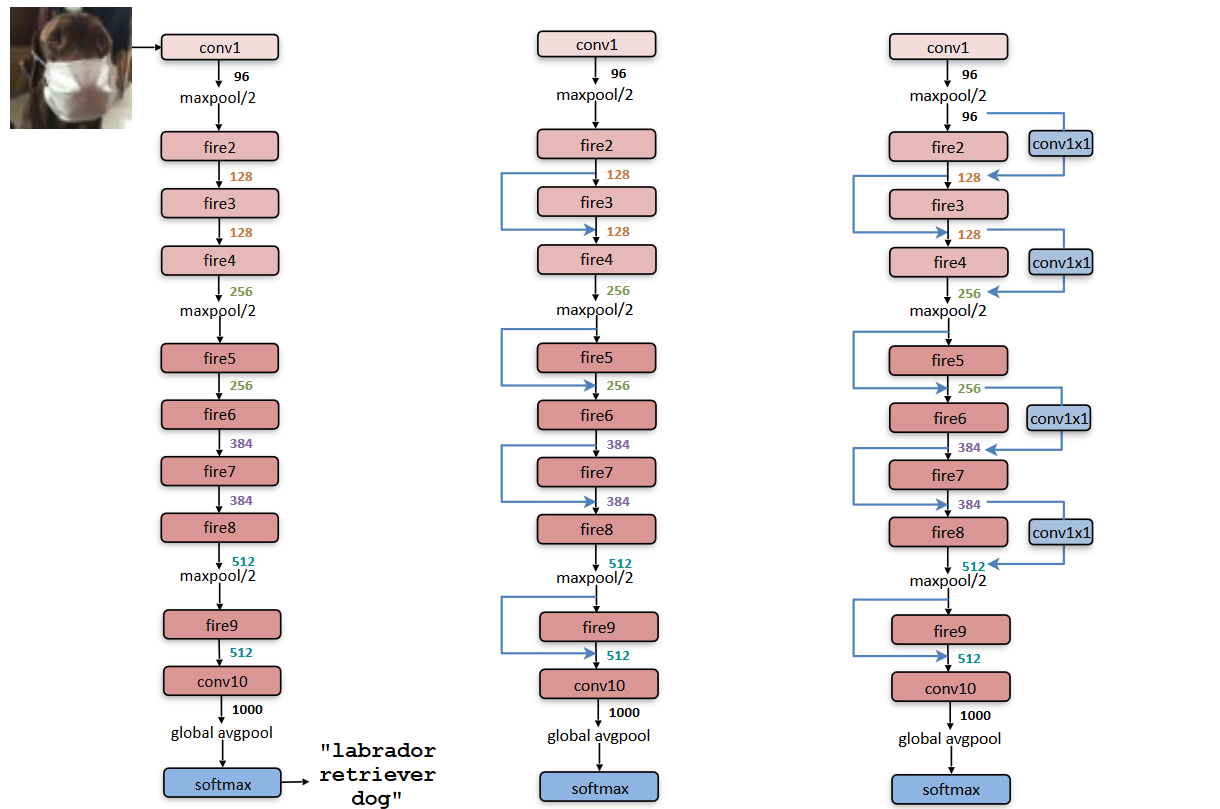
\includegraphics[scale=0.3]{../Images/squeezenetarch.png}
          \centering
          \caption{Macro architectural view of our SqueezeNet architecture. Left: SqueezeNet;
          Middle: SqueezeNet with simple bypass; Right: SqueezeNet with complex bypass}
        \end{figure}
      \subsubsection{MobiletNet (2017)}
        MobileNet represent both a class of efficient models for mobile and embedded vision applications and a streamlined architecture based on depth-wise separable convolutions to build lightweight CNNs.
        The principles behind this architecture are represented by two main components: \emph{Depthwise separable convolution} and a set of \emph{Hyperparameters}.

        Depthwise separable convolutions is a form of factorized convolutions which factorize a standard convolution into a depthwise
        convolution and a 1$\times$1 convolution called a pointwise convolution. For MobileNets the depthwise convolution applies a single filter to each input channel. The pointwise
        convolution then applies a 1$\times$1 convolution to combine the outputs the depthwise convolution. A standard convolution both filters and combines inputs into a new set of outputs
        in one step. The depthwise separable convolution splits this into two layers, a separate layer for filtering and a separate
        layer for combining. This factorization has the effect of drastically reducing computation and model size \cite{MNet}. A visual representation is shown in figure.

        \begin{figure}[H]
          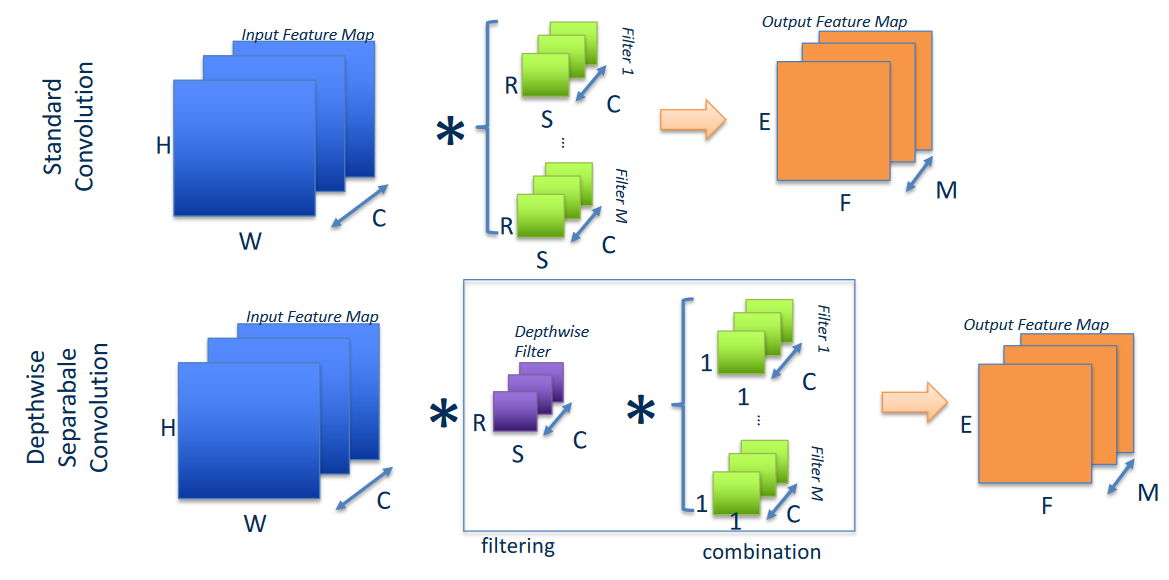
\includegraphics[scale=0.4]{../Images/DWConv.png}
          \centering
          \caption{Visual representation of Depthwise separable convolution}
        \end{figure}

        Following the figure notation we can compile a table comparing the memory and MACs requirements of the standard and the depthwise convolution:

        \begin{table}[H]
          \resizebox{\columnwidth}{!}{%
          \begin{tabular}{@{}ccc@{}}
          \toprule
          Type      & MACs                              & Memory            \\ \midrule
          Standard  & R $\times$ S $\times$ C $\times$ E $\times$ F $\times$ M             & R $\times$ S $\times$ C $\times$ M     \\ \midrule
          Depthwise & R $\times$ S $\times$ C $\times$ E $\times$ F + C $\times$ M $\times$ E $\times$ F & R $\times$ S $\times$ C + C $\times$ M \\ \midrule
          Ratio     & $\frac{1}{M}$ + $\frac{1}{R \times S}$                    & $\frac{1}{M}$ + $\frac{1}{R \times S}$   \\ \bottomrule
          \end{tabular}%
          }
          \centering
          \caption{Comparison between types of convolution}
        \end{table}

        As we can see the Depthwise separable approach allows us to have a considerable reduction in both MAC operations and number of weights. Moreover, with the help of the hyperparameters $\alpha$, or width multiplier, and $\rho$, or resolution multiplier, we can scale
        our model more efficiently acting directly on the number of filter ($\alpha$) and/or on the feature map size ($\rho$).

        The second revision of this family of network introduces the concepts of \emph{Linear Bottlenecks} and \emph{Inverted Residuals}.

        The first concept relies on the fact that our \emph{Manifold of Interest (MoI)}, where the interesting information resides, should be processed as part of a higher dimensional space (More channels) to avoid information loss when passing through a non-linear activation. This can be achieved
        efficiently by decompressing the input feature map with a pointwise convolution, then processing it, and at the end reducing the dimension using a linear bottleneck (a pointwise convolutional layer without activation). The expansion factor $t$ has an optimal value of 6 (experimental) and indicates
        how much the input should be expanded.

        The second concept is a simple bypass that helps the gradient propagate through the model. The nomenclature inverted comes from the fact that normally in other model residuals connections are made between thick layers while here the layer are thin.
        The following figure shows the structure of this module:
        \begin{figure}[H]
          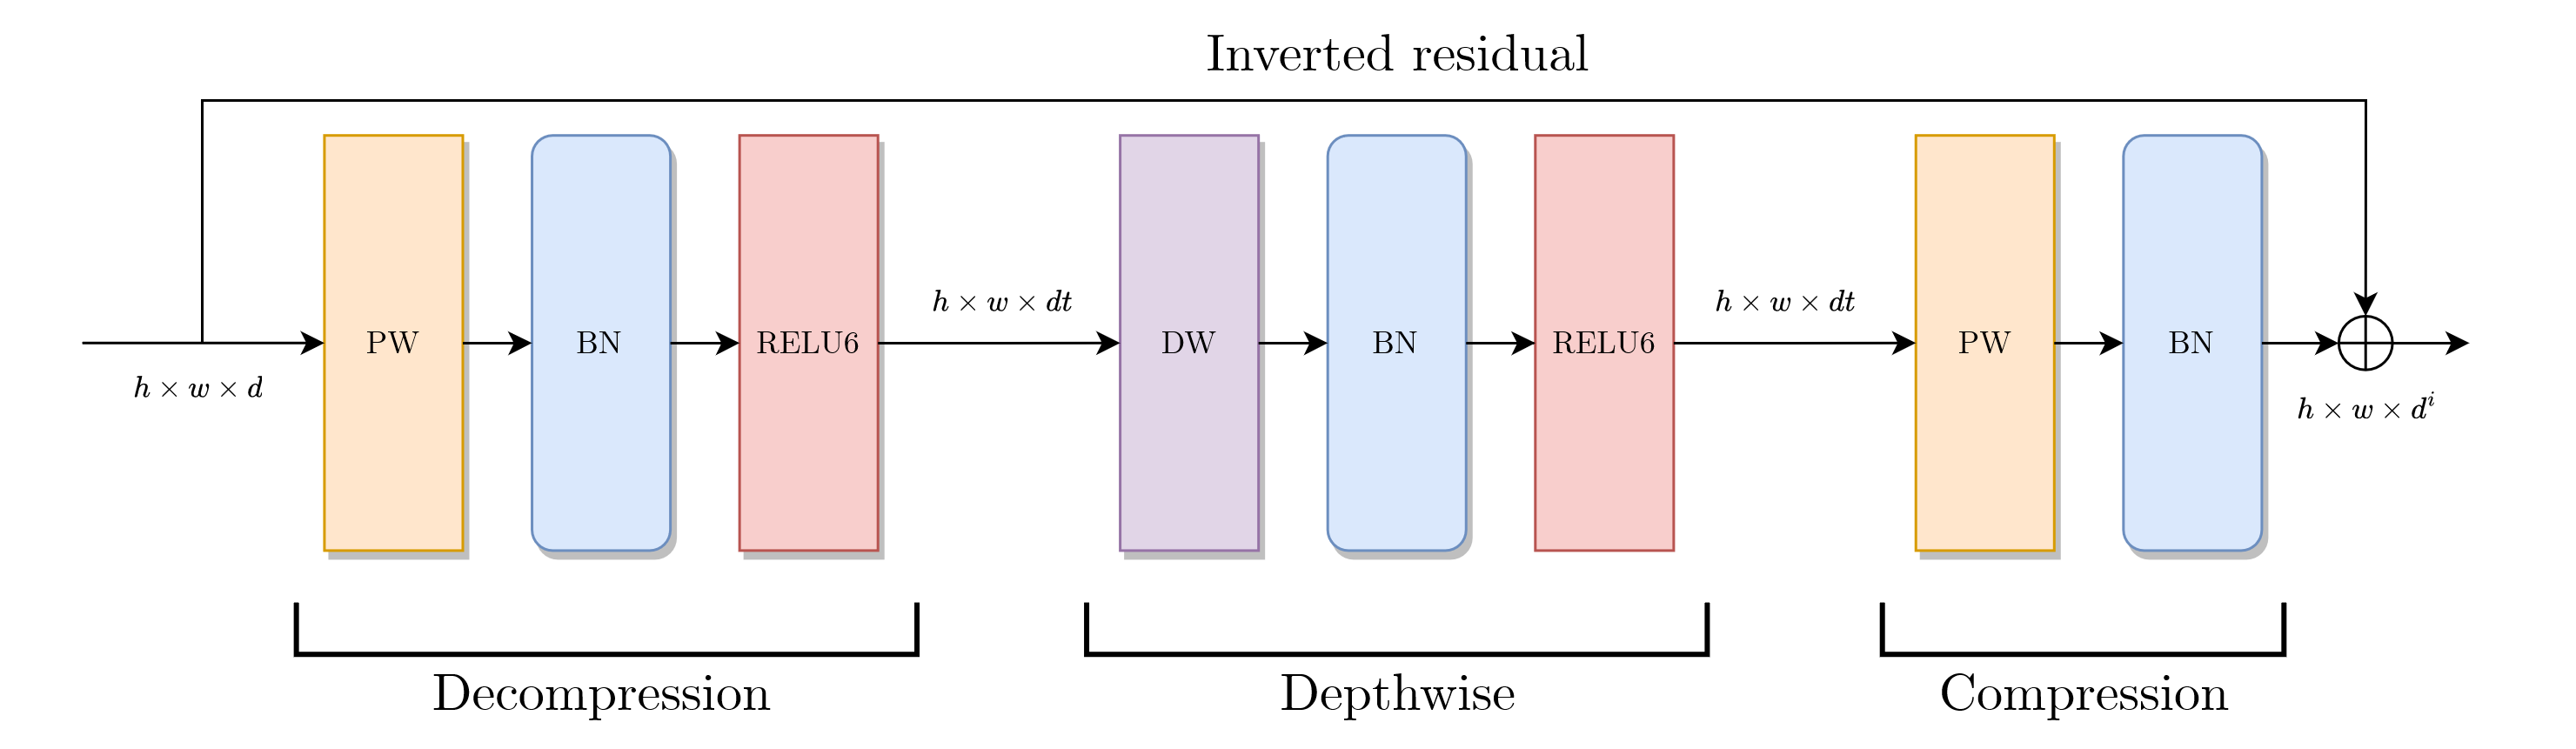
\includegraphics[scale=0.6]{../Images/MnetV2.png}
          \centering
          \caption{Linear bottleneck and inverted residual module}
        \end{figure}

        This allows us to reduce the number of filters for the intermediate layers, speeding up computations and decreasing the memory footprint. This second version is faster, smaller and more accurate than the first.
      \subsubsection{EfficentNet (2019)}
        The outstanding question now is how can we create scalable models to fit various technological constraints. A proposed solution is proposed in \cite{ENet} taking the name of EfficentNet. The goal is to 
        \emph{rethink model scaling for convolutional neural networks} in order to create efficient architectures and scaling mechanism.

        We can act on 3 main hyperparameters: the depth of the network $d$ (i.e. the number of layers), the width $w$ (i.e. the dimension of the intermediate feature maps) and the resolution $r$ (i.e. the input resolution).

        We empirically observe that different scaling dimensions are not independent. Intuitively, for higher resolution images, we should increase network depth, such that the larger receptive fields can help capture similar features that include
        more pixels in bigger images. Correspondingly, we should also increase network width when resolution is higher, in order to capture more fine-grained patterns with more pixels
        in high resolution images. These intuitions suggest that we need to coordinate and balance different scaling dimensions rather than conventional single-dimension scaling

        This creates the need for a \emph{Compound scaling mechanism} as shown in the next figure.
        
        \begin{figure}[H]
          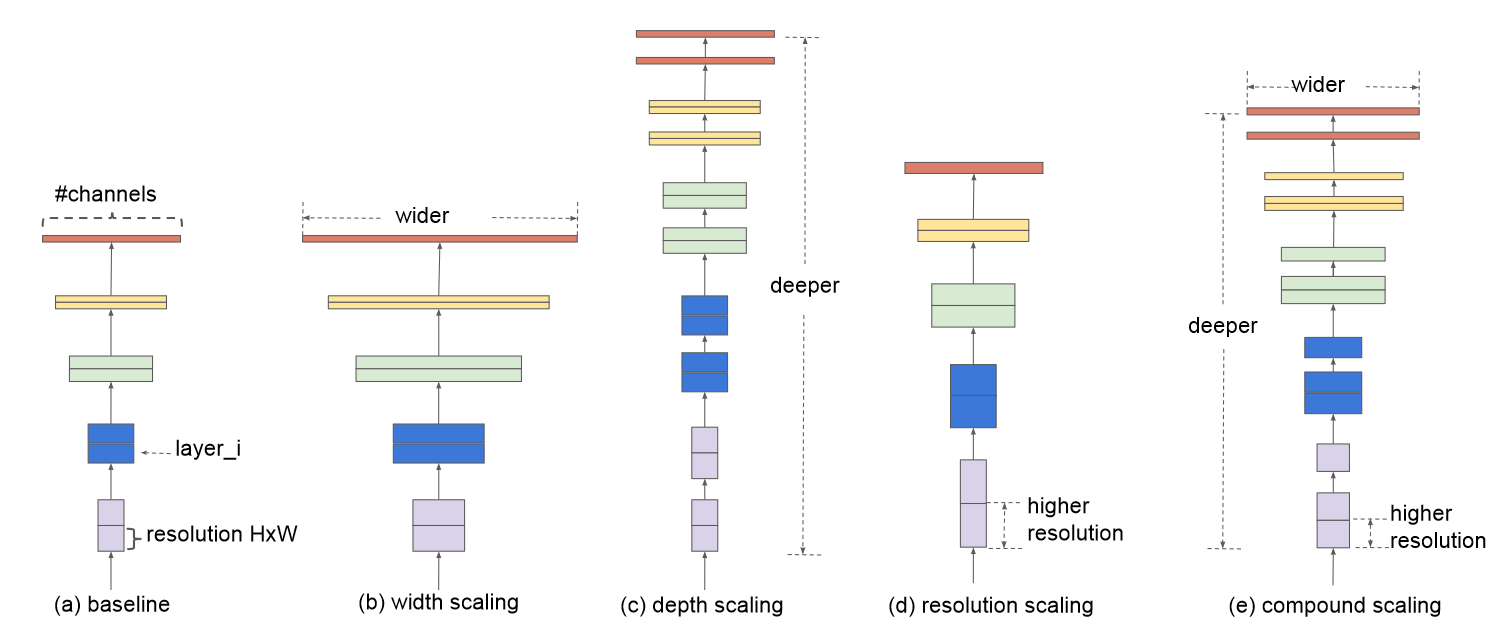
\includegraphics[scale=0.35]{../Images/ENetScaling.png}
          \centering
          \caption{Scaling of CNN}
        \end{figure}

        Defining now $\alpha, \beta, \gamma$ as constants and $\phi$ as user-specified coefficient controlling how many more resources are available for model scaling we can define as system of equation:

        \begin{equation}
          \left\{\begin{array}{cl}
            d & = \alpha^\phi \\
            w & = \beta^\phi  \\
            r & = \gamma^\phi
           \end{array}\right.
           \underrightarrow{with}
           \begin{array}{cl}
            &\alpha\cdot\beta^2\cdot\gamma^2 \approx 2 \\
            &\alpha \ge 1, \beta\ge 1,\gamma\ge 1
           \end{array}
        \end{equation}

        Now by setting $\phi =1$ setting a NN and assuming twice more resources available, a small grid search of $\alpha, \beta, \gamma$ is carried out, under the constraints. After we can use the resulting value of the constants
        and scale up the baseline network with different values of $\phi$. The result are quite good as shown in the next table.

        \begin{figure}[H]
          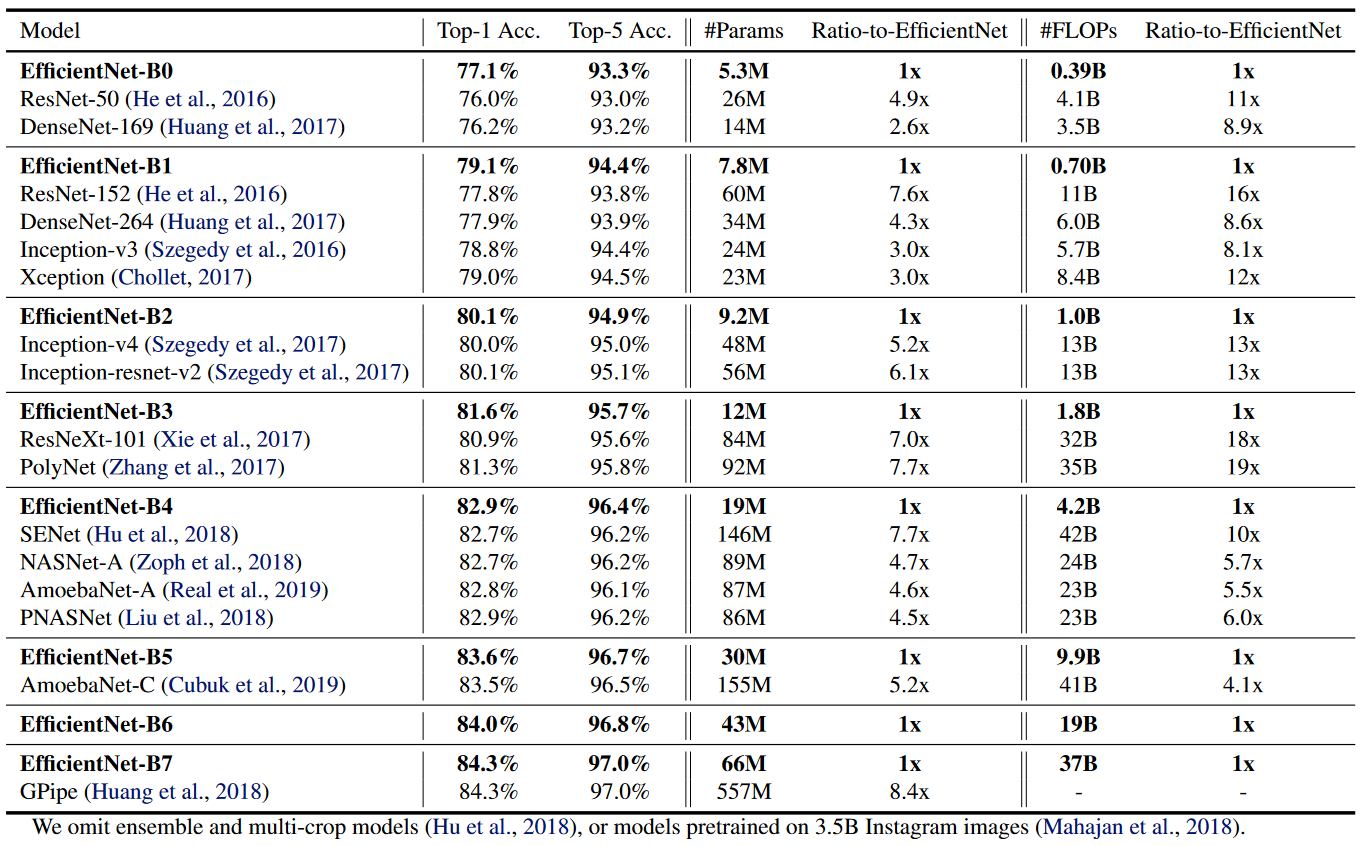
\includegraphics[scale=0.3]{../Images/EnetPreformance.png}
          \centering
          \caption{Performance of EfficentNet}
        \end{figure}
    \subsection{Approximate computing}
      Starting from the framework of an efficient neural network we can introduce the topic of \emph{Approximate Computing} to make our models fit the memory and computational requirements of tiny devices. There are two main approaches:
      \subsubsection{Quantization (Precision scaling)}
        Quantization is the process of reducing the memory occupation of the CNN by changing the precision of the weights (Number of bits for the representation). This procedure is carried out by a quantizer which can be implemented in a few different ways:

        \begin{itemize}
          \item \emph{Linear quantizer}: uniform distance between each quantization level (number of bits: 32, 16, 8 or custom)
          \item \emph{Log function}: the distance between the levels varies (e.g., log base2 quantization with logarithmic distribution of intervals). When weights are power of 2, multiplication maps into bit shifts
          \item \emph{Data-driven}: quantization levels are determined or learned from the data, e.g., using k-means clustering.
        \end{itemize}

        The specific implementation depends on the distribution of weights as shown in figure:
        \begin{figure}[H]
          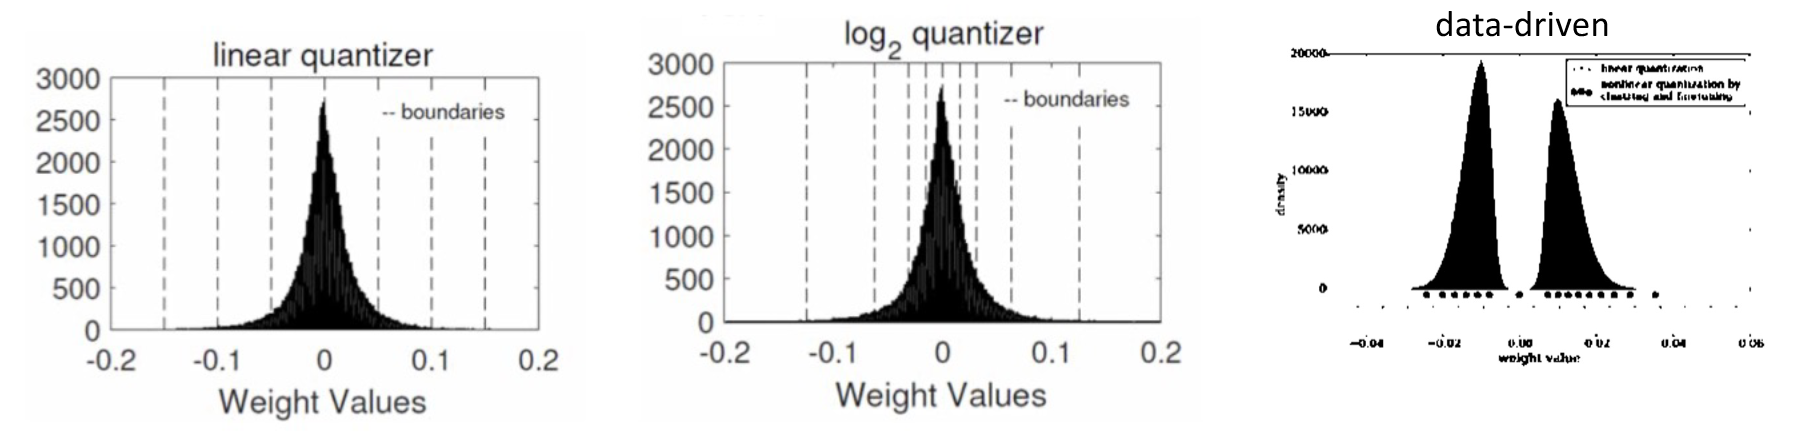
\includegraphics[scale=0.3]{../Images/WeightDistribution.png}
          \centering
          \caption{Different quantizer implementations}
        \end{figure}

        Inside the model we can quantize both the weights (reducing the memory requirements) and the activations (effect depends on the network). Additionally, we can apply Variable quantization with different quantization mechanics (w.r.t. layers) instead of a fixed quantization policy.

        The performance loss attributed to quantization varies from model to model, but we can take AlexNet as a case study.
        \begin{figure}[H]
          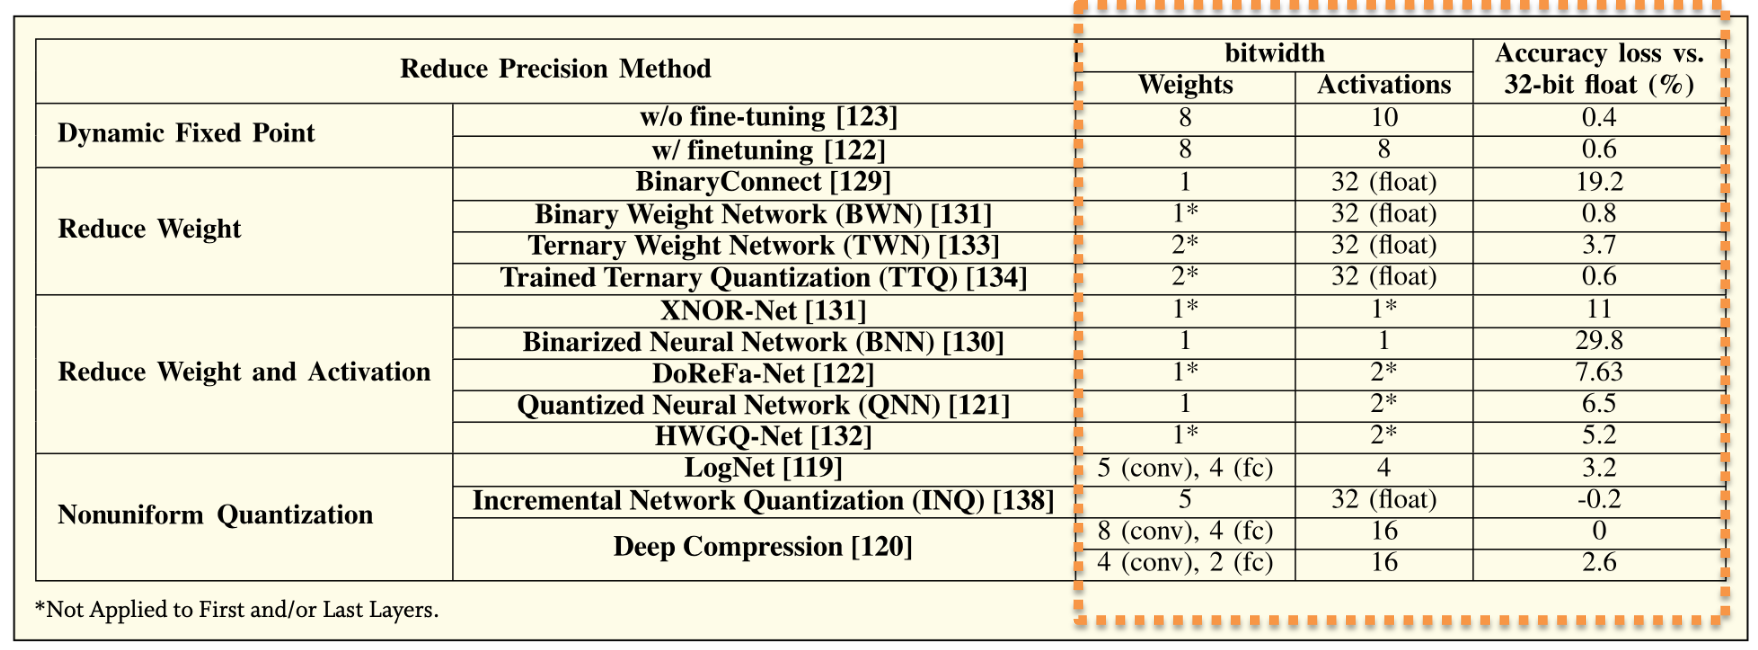
\includegraphics[scale=0.3]{../Images/QuantizationPerformance.png}
          \centering
          \caption{Quantization performance loss on AlexNet}
        \end{figure}

        As we can see the performance loss in very small for conservative quantization. It is important to point out that even if extreme quantization methods are listed we are limited by the specific software implementation, since most microcontrollers and devices support a minimum of 8-bit for data type.

        Still, it is interesting how the ternary network $(-w, 0, w)$ for which a different scale is trained for each weight, exhibits only a $0.6\%$ loss.

        In general 8-bit quantization allows for a reduction of 3x to 30x energy with respects to an add operation and of 15.5x to 18.5x with respects to a multiply operation while also allowing for 4 operation in one system clock cycle. 

        In the implementation we need to specify 3 parameters: the bit width $b$, the scale factor $s$ and the zero-point $z$ (only necessary for asymmetric quantization). The scale factor and the zero-point are used to map a floating point value to the integer grid,
        whose size depends on the bit-width. The scale factor is commonly represented as a floating-point number and specifies the step-size of the quantizer.
        The zero-point is an integer that ensures that real zero is quantized without error.
        For asymmetric quantization the quantized value results in:
        
        \begin{equation}
          x_{int} = clamp(\left\lfloor \frac{x}{s}  \right\rceil + z ; 0 ; 2^b-1) \rightarrow 
          clamp(x,a;b)= \left\{\begin{array}{cl}
            a, & x < a \\
            x, & a \le x \le b  \\
            b, & x>c
           \end{array}\right.
        \end{equation}

        To dequantize we can use:

        \begin{equation}
          x \approx \hat{x} = s(x_{int}-z) \in
          [q_{\min};q_{\max}] \rightarrow \left\{\begin{array}{cl}
            q_{\min}= & -sz \\
            q_{\max}= & s(2^b-1-z) 
           \end{array}\right.
        \end{equation}

        Intuitively any value that falls out of the range$ [q_{\min};q_{\max}]$ will result in clipping error. We can reduce this by increasing the scale factor s allowing the expansion of the quantization range.
        However, increasing the scale factor leads to an increased rounding error $\epsilon_r \in [-\frac{s}{2};\frac{s}{2}]$

        \begin{figure}[H]
          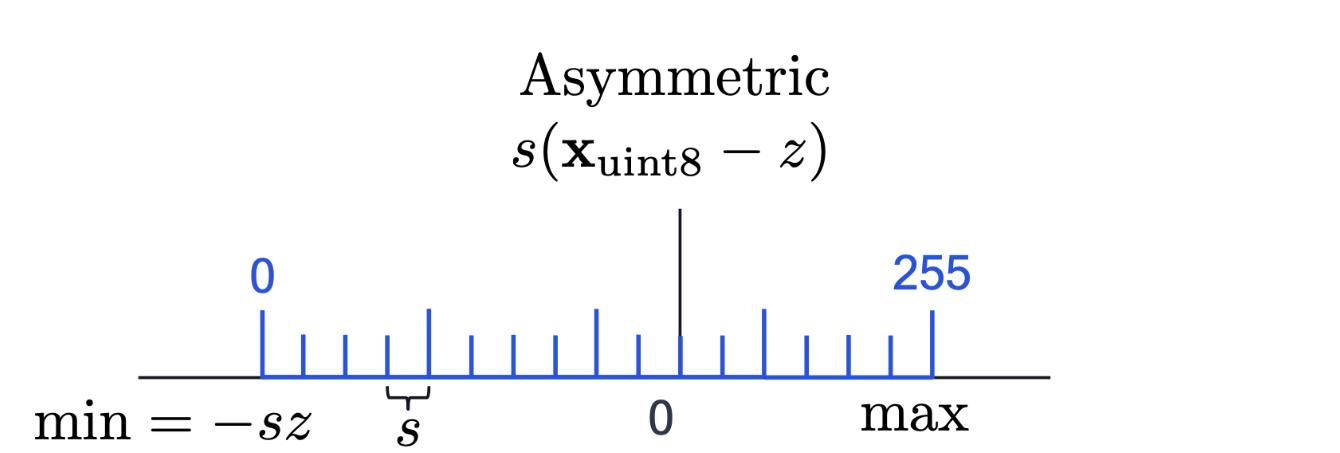
\includegraphics[scale=0.3]{../Images/AsimmQuant.png}
          \centering
          \caption{Asymmetric quantization}
        \end{figure}

        Symmetric quantization is simpler, showing both signed and unsigned version:
        
        \begin{equation}
          \begin{array}{cll}
            x_{int} = &clamp(\left\lfloor \frac{x}{s}  \right\rceil; 0 ; 2^b-1) &for\ unsigned\ integers \\
            x_{int} = &clamp(\left\lfloor \frac{x}{s}  \right\rceil; -2^{b-1} ; 2^{b-1}-1) &for\ signed\ integers
          \end{array}
        \end{equation}

        While the dequantization step is simply $\hat{x}=sx_{int}$.

        \begin{figure}[H]
          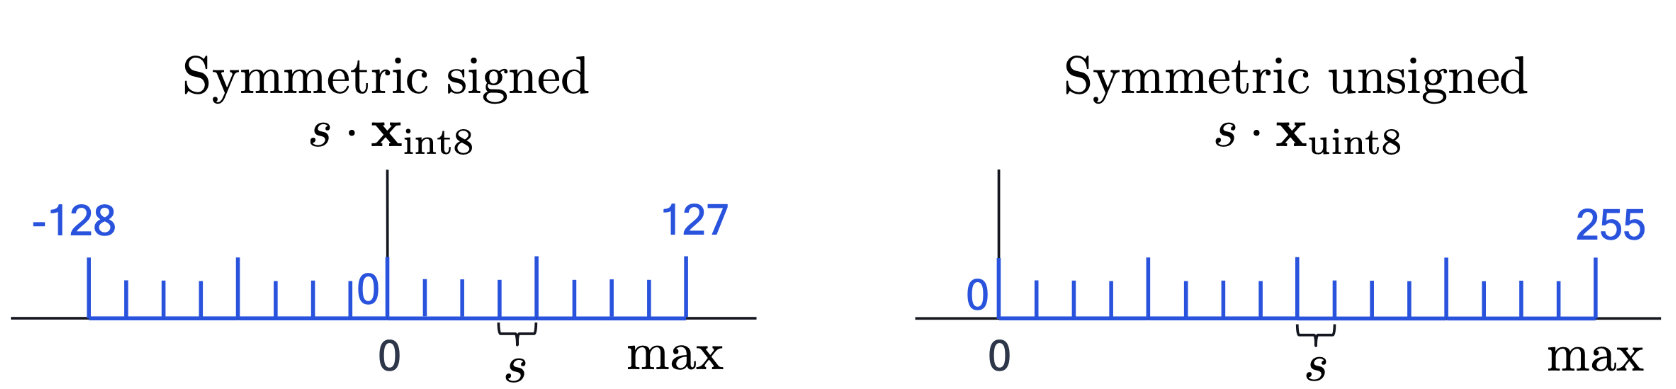
\includegraphics[scale=0.3]{../Images/SimmQuant.png}
          \centering
          \caption{Symmetric quantization}
        \end{figure}

        Using the Symmetric quantization as an example we can write the quantized version of a MAC operation as:
        \begin{equation}
          \begin{array}{cl}
            \hat{A}_n & = \hat{b}_n + \sum_{m}^{} \hat{W}_{m,n} \hat{x}_m \\
                      & = \hat{b}_n + \sum_{m}^{} (s_w W_{n,m}^{int})(s_x x_{m}^{int}) \\
                      & = \hat{b}_n + s_w s_x \sum_{m}^{} W_{n,m}^{int}x_{m}^{int}
          \end{array}
        \end{equation}

        Where we employ two different scale factors for weights and activations. The result need to be requantized due to add operation.

        \begin{figure}[H]
          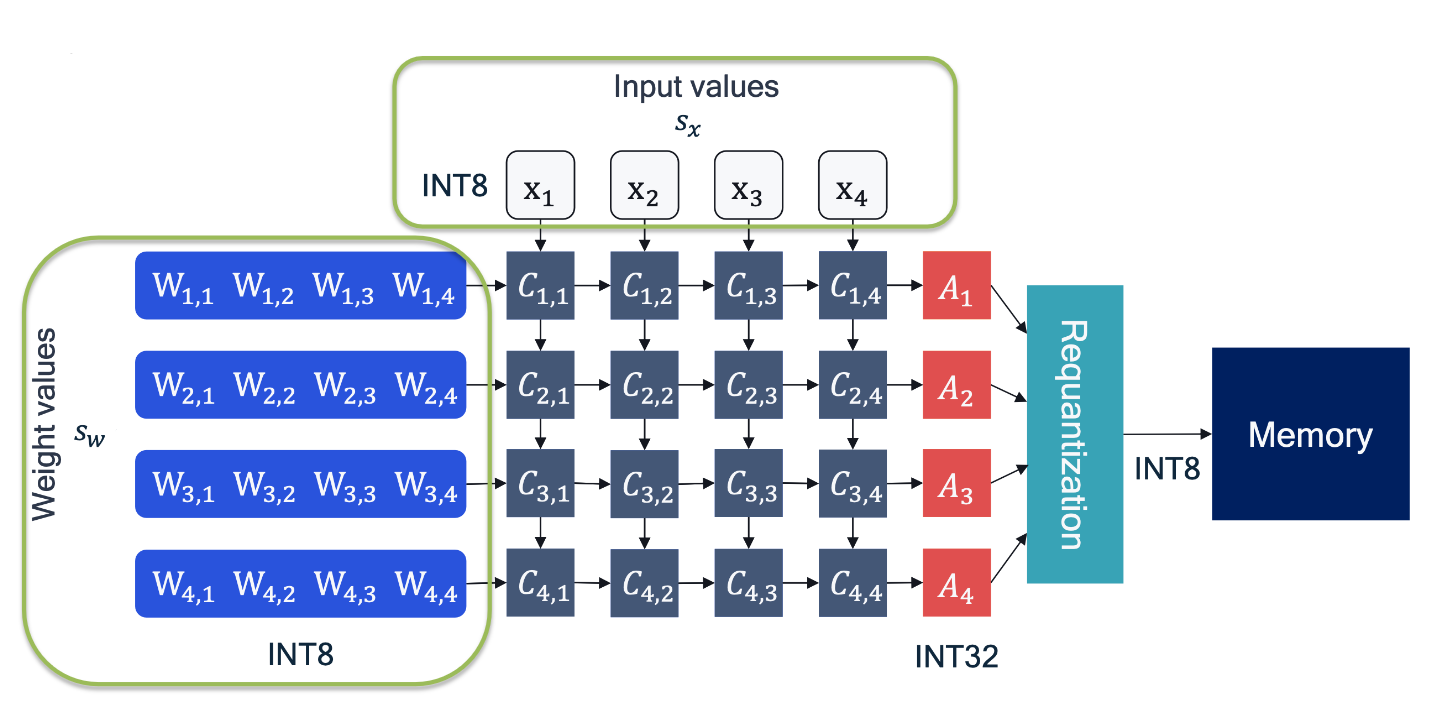
\includegraphics[scale=0.3]{../Images/MatrixQuant.png}
          \centering
          \caption{Example of quantized operation}
        \end{figure}

        Finally, we must choose between:
        \begin{itemize}
          \item Post-training: quantization (PTQ): a pre-trained FP32 network is directly converted into a fixed-point network without the need for the original training pipeline.
          The main challenge is the definition of the quantization range settings. Two main approaches: 
          \begin{equation}
            \begin{array}{ll}
              MinMax & = [q_{\min};q_{\max}] = [\min V;\max V] \\
              MSE     & = \underset{q_{\min},q_{\max}}{argmin} \ \left\| V-\hat{V}(q_{\min},q_{\max}) \right\|_F^2
            \end{array}
          \end{equation}

          This approach is effective and fast to implement since they do not require retraining of the network with labeled data, but offers limited performance when low-bit quantization of activations (e.g., 4-bit and below) is considered
          and due to high rounding errors when considering wide ranges. Also, post-training techniques may not be enough to mitigate the large quantization error incurred by low-bit quantization.
          
          \item Quantization-aware training (QAT): quantization and training are jointly addressed (back-propagation implemented with simulated quantization within the training pipeline). Here higher accuracy comes with the usual costs of neural network training,
          i.e., longer training times, need for labeled data and hyperparameter search. Now the challenge is how to back-propagate through the simulated quantizer block. The solution is to approximate the gradient using the straight-through
          estimator (Bengio et al. 2013), which approximates the gradient of the rounding operator as 1 ($\frac{\partial \left\lceil  y\right\rfloor }{\partial y} = 1$)
          \begin{figure}[H]
            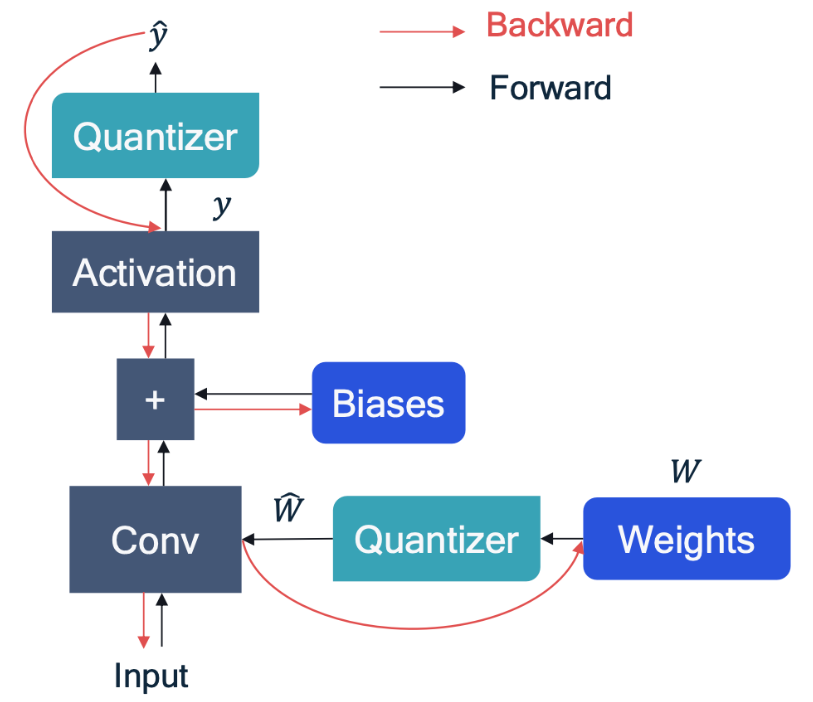
\includegraphics[scale=0.3]{../Images/QAT.png}
            \centering
            \caption{Quantization-aware training (QAT)}
          \end{figure}
        \end{itemize}
      \subsubsection{Task Dropping}
        Task dropping is the process of reducing the computational load and the memory occupation by skipping the execution of some tasks associated with the processing chain. We want to reduce the number of operations and model size. This might have
        a positive effect on computational demand and memory footprint. We have a wide range of techniques such as:
        \begin{itemize}
          \item Network pruning: Usually, to allow easier training, Neural Networks are over parameterized. As a result, a large amount of the weights in a network is redundant
          and can be removed (i.e., set to zero). However, aggressive network pruning often requires some fine-tuning of the weights to maintain the original accuracy.

          This procedure can be carried out in a more structured manner by pruning entire group of weights (entire row, entire column, filters, etc.).
          \item Network architecture design: In most networks we can replace a large filter with a series of small filters, either before training, by switching from 5$\times$5 to 3$\times$3 filter and decomposing a N$\times$N in a combination of 1$\times$N and N$\times$1,
          or after training, by employing tensor decomposition (to decompose filters without impacting accuracy), low rank approximation and canonical polyadic decomposition.
          \item Transfer Learning: In a general setting we can take an existing pre-trained network, cut the last $k$ layer and replace them with a unique processing layer. This will allow us to get an application-specific and approximated CNN without the training overhead required to retraining the whole network.
          In layman terms we are keeping the weights of only part of the network.
          \item Knowledge distillation: In this approach we employ two models, a bigger pre-made \emph{Teacher model} and our smaller \emph{Student model}. We can now use the combined Cross-entropy gradient to update the network. The combined gradient can be expressed as:
          \begin{equation}
            \frac{\partial C}{\partial z_i} = \frac{1}{T} (q_i -p_i) = 
            \frac{1}{T} (\frac{e^{\frac{z_i}{T}}}{\sum_{j}^{}e^{\frac{z_j}{T}}}-
            \frac{e^{\frac{v_i}{T}}}{\sum_{j}^{}e^{\frac{v_j}{T}}})
          \end{equation}
          \begin{figure}[H]
            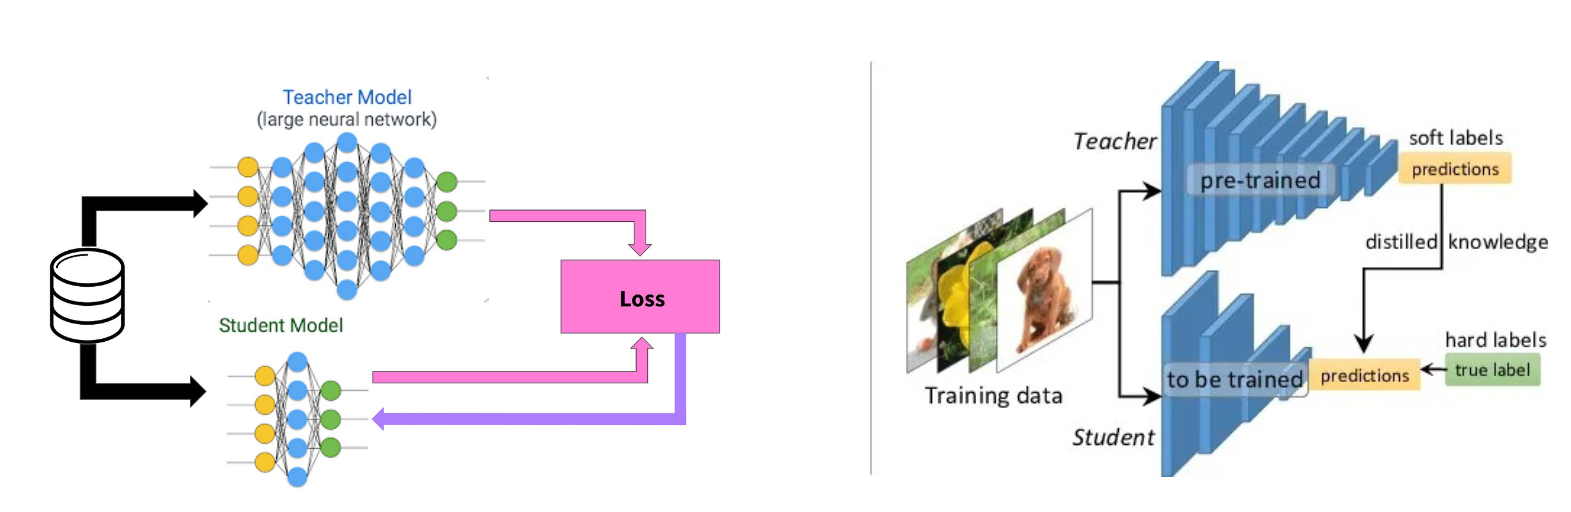
\includegraphics[scale=0.25]{../Images/KnowledgeDistillation.png}
            \centering
            \caption{Knowledge distillation}
          \end{figure}
        \end{itemize}
      \subsubsection{Summary}
      In summary, we can define a tool chain as shown in the next figure:
      \begin{figure}[H]
        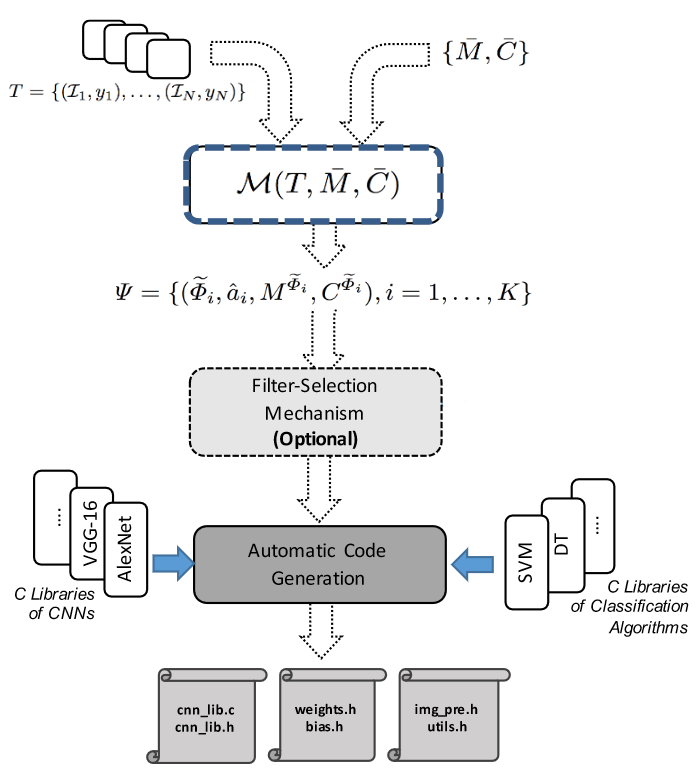
\includegraphics[scale=0.25]{../Images/OptToolchain.png}
        \centering
        \caption{Tiny Model tool chain}
      \end{figure}

      Where $M$ receives in input a dataset $T$ and the constraints on memory $M$ and computation $C$. Its output is the Pareto set of satisfying the constraints on $M$ and $C$.
      The Filter-Selection Mechanism then identifies those filters providing output features that are truly beneficial to support the classification by $\mu$ and discard the others.
      As we can see in the next figure this can efficiently scale down a network to make it run decently even on a microcontroller:
      \begin{figure}[H]
        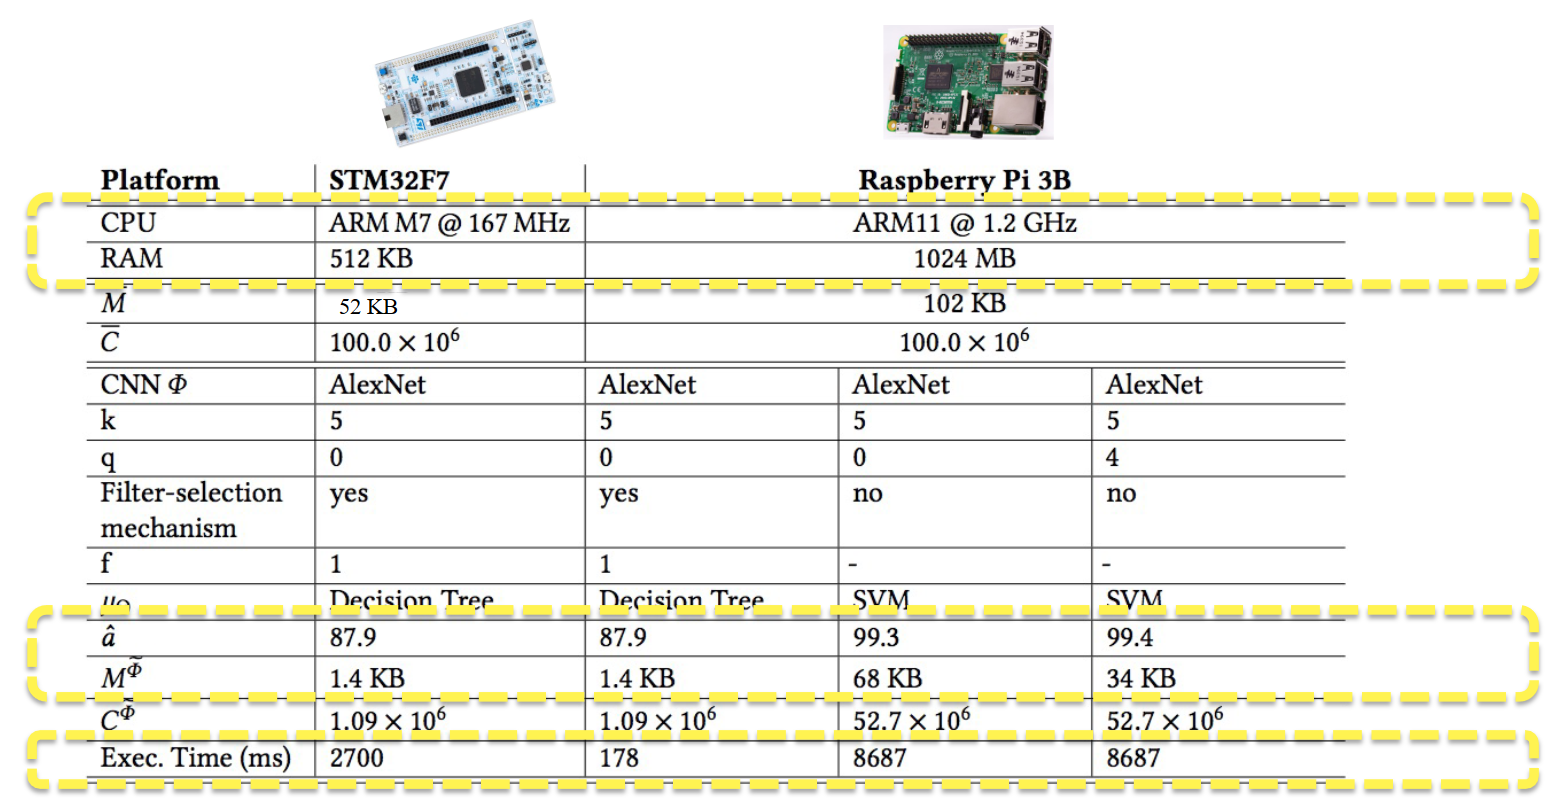
\includegraphics[scale=0.35]{../Images/OptResults.png}
        \centering
        \caption{AlexNet approximation results}
      \end{figure}
        


    \subsection{Embedded system code optimization}

  \section{Early Exit Neural Networks (EENN)}
    Until now, we have designed Neural Networks as a stack of layers, in which a result is obtained only after processing the full stack. While this approach is straightforward it can lead to Over-parameterization, Extended latency and memory constraints and
    Over-learning (it might happen, for long pipelines, that at different points of the processing the decision changes for the worst, a shorter pipeline could fix this).

    The rationale here is to understand that, for some tasks, we need only part of the model, extracting a meaningful output before the end of the pipeline. To correctly apply this we need to incrementally process the input through the model layers and take a
    decision as soon as \emph{enough confidence} is gained.

    To correctly employ this we can take the original network (In this scope referred as \emph{Backbone network}) and insert additional small classifier (\emph{Early Exit Classifiers or EECs}) in various point of the pipeline, creating an EENN.

    This lead to the mitigation of many drawbacks of DNNs such as overfitting, vanishing gradient and overthinking as well as offering a significant reduction of the inference time. The idea also adds the capability of being distributed over multi-tier computation platforms by 
    enhancing the adaptiveness to changing environments by achieving a desired trade-off between accuracy and efficiency on the fly. By having multiple outputs we also increase the interpretability of the network (since we can analyze each decision individually).

    This all makes sense if we draw a parallel between human behavior and our models. In fact, some decisions might be better if we don't overthink them. This directly translates in what we discussed earlier.
    \subsection{EECs and the selection scheme}
      We can implement an EENN by simply considering that for each intermediate layer output $f_i(x)$ we can define  small classifier (EEC) such that the intermediate decision at layer $i$ is:
      \begin{equation}
        \overline{y}_i = C_i(f_i(x)) 
      \end{equation}

      In this way we now have a sequence of predictions, but how do we choose which prediction to use? In short an input sample exits from an EEC when enough confidence is achieved, in this case the sample is not forward propagated (the network makes an early exit). The decision is taken by the \emph{selection scheme} which is a set of decision functions.

      This class of function simply compares the confidence value $C_i$ with a corresponding threshold $\theta_i$ that sets the minimum confidence to take the decision. In formulas:

      \begin{equation}
        D_i(x) = C_i(x)\geq \theta_i \ , \  i \in [1,N_l] \ , \ \theta \in [0,1]
      \end{equation}

      \begin{quote}
        Note that for $\theta = 0$ the network always makes an early exit, while for $\theta = 1$ the network will never exit at that node.
      \end{quote}

      \begin{figure}[H]
        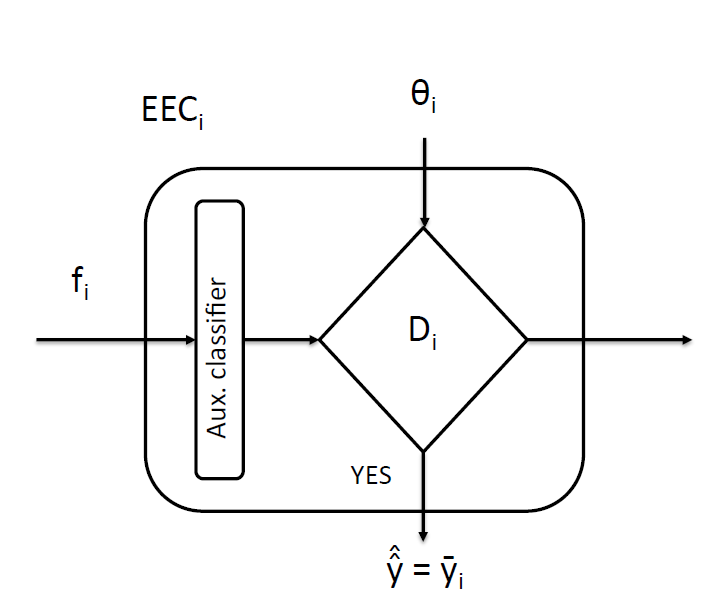
\includegraphics[scale=0.35]{../Images/EEC.png}
        \centering
        \caption{Early Exit Classifier}
      \end{figure}

      For classification problems, a popular approach for EENNs relies on ability to estimate the confidence of the neural network on its own prediction and use it to decide whether to early exit the processed input. The confidence value can be measured mainly in three ways:
      \begin{itemize}
        \item \emph{Max Softmax output}: By directly taking the output of the softmax of the EEC we can select the class with the maximum probability and compare it to the threshold. This is a direct measure of confidence (The network does not exit if the probability is less that $\theta$).
        \item \emph{Score Margin}: The score margin (SM) is the distance between the largest and the second-largest value of the softmax output. Intuitively, the higher the “confidence” of the EEC i about its
        prediction, the higher the difference between the largest and the second-largest value. This is still directly comparable to the threshold.
        \begin{figure}[H]
          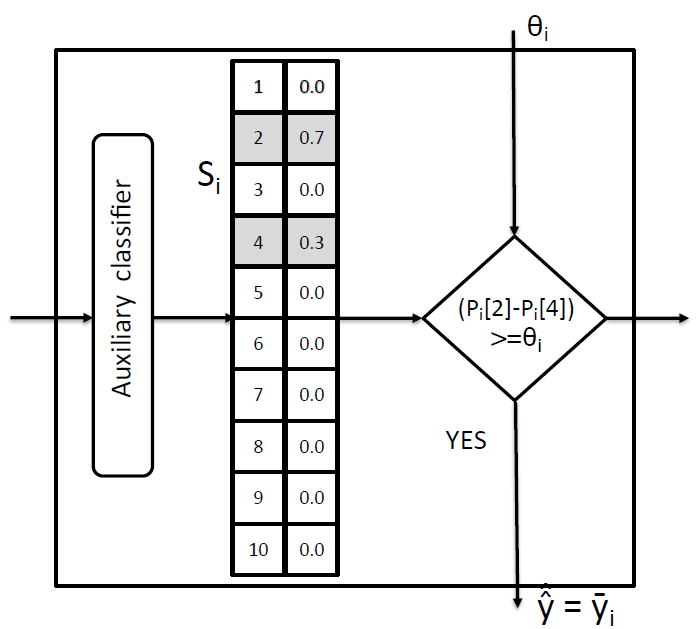
\includegraphics[scale=0.35]{../Images/SM_EEC.png}
          \centering
          \caption{Score Margin Example}
        \end{figure}
        \item \emph{Entropy}: The entropy H estimates the level of uncertainty on the prediction:
        \begin{equation}
          H(y) = \sum_{i=0}^{N} y_i * \log(y_i)
        \end{equation}
        The entropy is minimal whenever y equals a one-hot vector, and maximal when it is equal to a uniform distribution over classes.
      \end{itemize}
    \subsection{Training of EENN}
      The training EENNs can be categorized into three main families:
      \begin{itemize}
        \item \emph{Joint Training (JT)}: Consists in jointly training all the EECs by combining the loss of the classifier as:
        \begin{equation}
          L_{joint} = L(\hat{y},y) +\sum_{i=1}^{N} w_i * L(\hat{y_i},y)
        \end{equation} 
        Where $L$ is the standard Cross Entropy loss and $N$ is the number of EECs. The weights $w_i$ can be set to 1 or become hyperparameters. This extends the time needed to converge as well as the data needed but trains everything at the same time.
        \begin{figure}[H]
          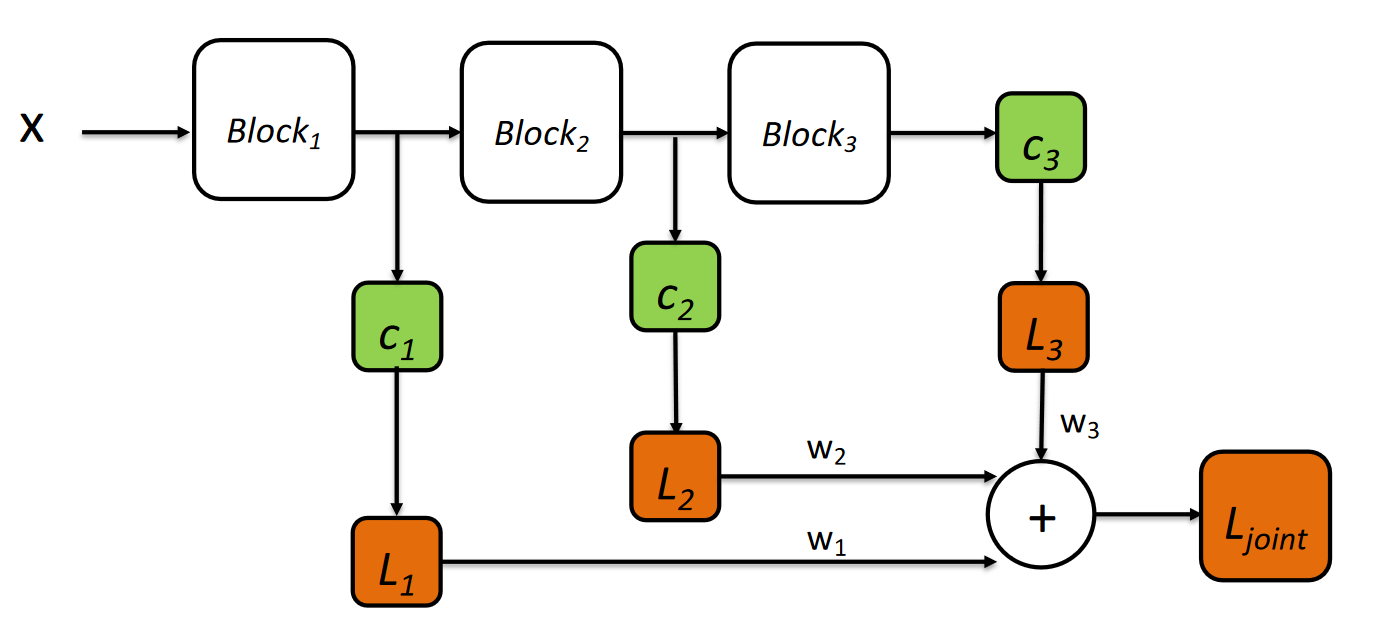
\includegraphics[scale=0.35]{../Images/JointTraining.png}
          \centering
          \caption{Joint Training}
        \end{figure}
        
        \item \emph{Layer-Wise Training (LT)}: trains iteratively one block of the backbone network and the corresponding EEC keeping frozen the former pipeline of the neural network. This does not allow each block to be the optimal feature extractor, but
        we only need to train one block and one EEC. 
        \item \emph{Knowledge Distillation (KD)}: initially trains the backbone network (teacher) and, then, the EECs (students) on top of the trained backbone network. This just means training as usual and the using the backbone as is to train the EECs. This allows for training decoupling.
        \begin{quote}
          \centering
          Different from previous Knowledge Distillation!
        \end{quote}
      \end{itemize}
    \subsection{Inference of EENN}
      We can approach inference in two ways:
      \begin{itemize}
        \item The most trivial approach is to aggregate the outputs of all the EECs to provide a joint prediction. This is a sort of \emph{Fake EENN} since it compensates the overthinking issue by factoring in the previous decisions but does not provide any computational advantage.
        \item The most interesting approach is to process the input up to a given EEC and then, stop the forward propagation. This is the true reference inference scheme for EENNs.
      \end{itemize}
   
  \section{Learning in presence of concept drift}
    Up to now we assumed the system model to be stationary and time invariant but everything and everybody changes over time. These concepts can be defined formally if consider a data generating process:
    \begin{itemize}
      \item \emph{Stationarity}: We say that a data generating process is stationary when generated data are $i.i.d.$ realizations of a unique random variable whose distribution does not change with time. This constraint is violated if the \emph{pdf} of the data changes over time.
      \item \emph{Time invariance}: We say that a process is time invariant when its outputs do not explicitly depend on time. A time-invariant system for example is an AR model:
      \begin{equation}
        y(t)= a_1 y(t-1) + a_2 y(t-2) + \beta \ , \ \beta = N(0,\sigma^2)
      \end{equation}
      While a time-variant:
      \begin{equation}
          y(t)= a_1e^{t_0 -t}y(t-1) + a_2y(t-2) + \beta \ , \ \beta = N(0,\sigma^2)
      \end{equation}
    \end{itemize}

    Given that our machine learning models are built with these assumptions in mind, we must search for \emph{Adaptation}, which in a way mimics the human behavior. Now we have two main problems: \emph{What} we need to do to adapt and \emph{When} we want to do it.

    To answer the \emph{What} question we propose a series of methods:
    \begin{itemize}
      \item \emph{Instance Selection}: The idea is to identify the samples of the training set that are relevant to the current state of the process. Or in other terms to periodically change the training set to correctly adapt to the current scenario. The adaptive systems generally rely on a 
      window over the most recent training samples to process the upcoming data which can either be:
      \begin{itemize}
        \item \emph{Fixed}: the length of the window is fixed a-priori by the user.
        \item \emph{Heuristic}: adapt the window length over the latest samples to maximize the accuracy
      \end{itemize}
      While this method is easy to implement (low computational-complexity, reduced training set) it is also very memory hungry (We need to store the entire training set), requires a complete retraining of the model and introduces the problem of choosing the window size. Moreover, how do we choose when to change the training set?
      \begin{figure}[H]
        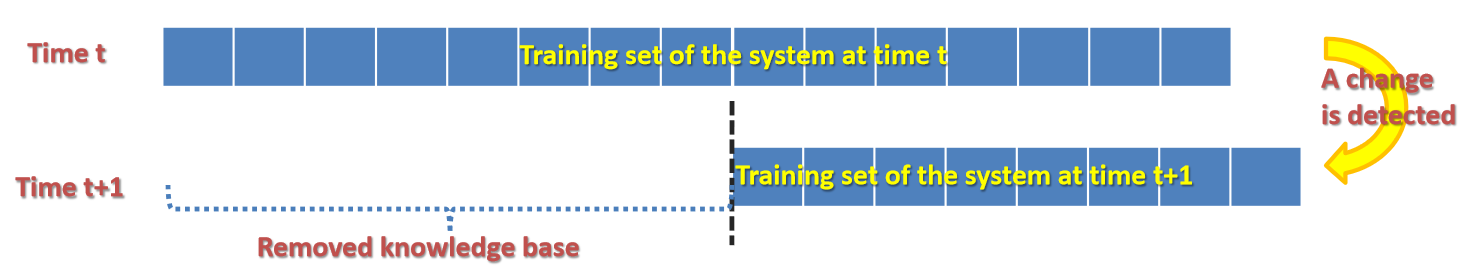
\includegraphics[scale=0.35]{../Images/InstanceSelection.png}
        \centering
        \caption{Instance Selection}
      \end{figure}
      \item \emph{Instance Weighting}: The idea is that training samples are not removed from the training set of the system but all the training samples (suitably weighted) are considered. The training samples might be weighted according to the age or
      the relevancy to the current state of the process in terms of accuracy of the last batch of supervised data.
      \begin{figure}[H]
        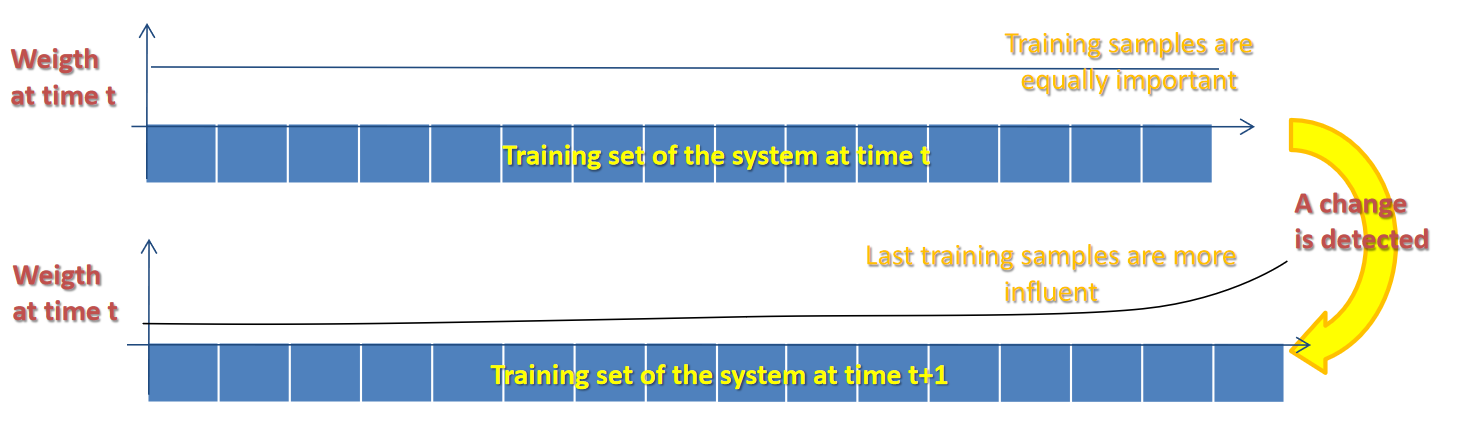
\includegraphics[scale=0.35]{../Images/InstanceWeight.png}
        \centering
        \caption{Instance Weighting}
      \end{figure}
      While this approach is still simple (low computational-complexity) and allows for all the training samples to be present at the same time is even more memory hungry and still require heuristic to define the sample weights. 
      \item \emph{Multiple Models}: The idea is that the outputs of an ensemble of models is combined by means of voting or weighted mechanisms to form the final output. All these systems includes techniques for dynamically including new models in the system or deleting
      obsolete ones (i.e., pruning techniques aiming at removing the oldest model or the one with the lowest accuracy).
      \begin{figure}[H]
        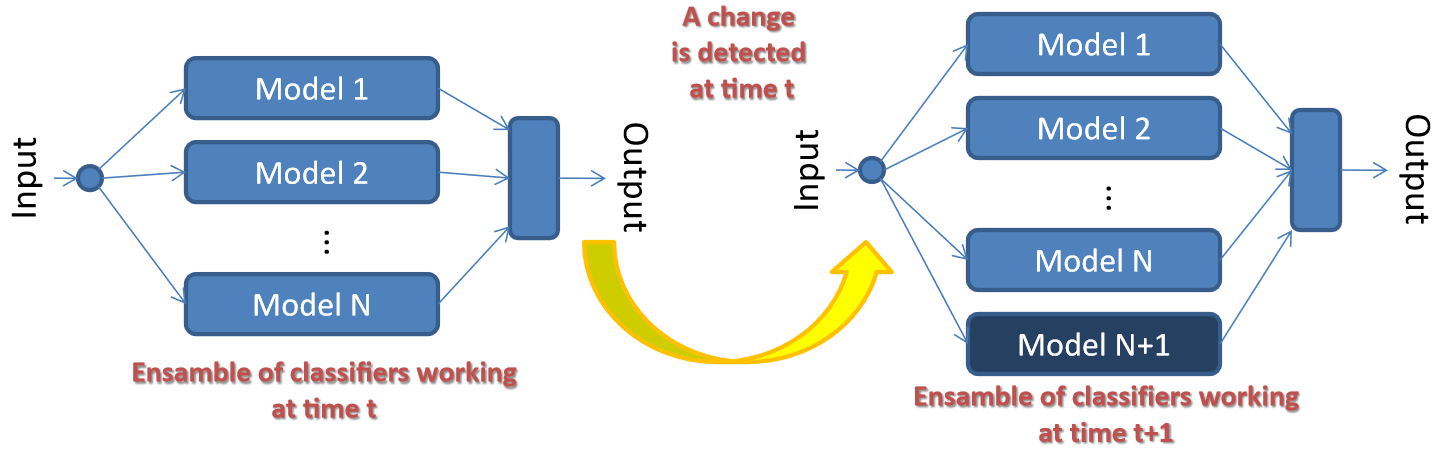
\includegraphics[scale=0.35]{../Images/MultipleModels.png}
        \centering
        \caption{Multiple Models}
      \end{figure}
      While this approach allows us to have a model for each bunch of data it comes at the price of high computational complexity.
    \end{itemize}

    To answer the \emph{When} question instead we need to distinguish between two main approaches
    \subsection{Passive approach}
      Passive solutions continuously adapt the model without the need to detect the change. This translates in ensembles of models with the adaptation phase consisting in a continuous update of the weights
      of the fusion/aggregation rule and creation/removal of models. This approach guarantees that the best model is always available but introduces a continuous overhead.

      The general idea that the underlying data distributions may (or may not) change at any time with any rate of change, so we employ continuous adaptation of the model parameters every time new data arrive to maintain an up-to-date model at all times and
      avoid the potential pitfall associated with false alarms in active solutions. Some solutions may include:
      
      \emph{Passive Learning} where for each new data point or batch of data we update the weights of the model.
      
      \emph{Ensemble learning} which provides a natural fit to the problem of learning in non-stationary environments. This approach is more accurate than single classifier-based systems, can easily incorporate new data into a classification model (a new item into the
      ensemble) and provide a natural mechanism to forget irrelevant knowledge (removing an item from the ensemble). Some implementations are:
      \begin{itemize}
        \item \emph{Streaming ensemble algorithm (SEA)}: where new classifiers are added as new batches of data arrive, until we reach a user-defined maximum number of classifiers, at which point we start removing some of them based on the evaluation of classifier’s predictions,
        the age of the classifier or by simply removing the least contributing member.

        \item \emph{Dynamic weighted majority (DWM)}
        \item \emph{Online bagging/boosting}

      \end{itemize}
    \subsection{Active approach}
      Active solutions rely on triggering mechanisms (oracle) to identify changes in the process and react by updating the model. This trigger can either monitor the pdf of the inputs (does not require labels, may ignore changes in performance), or the classification error (w.r.t. the nominal values) which is more challenging due to the need of labeled information.
      \begin{figure}[H]
        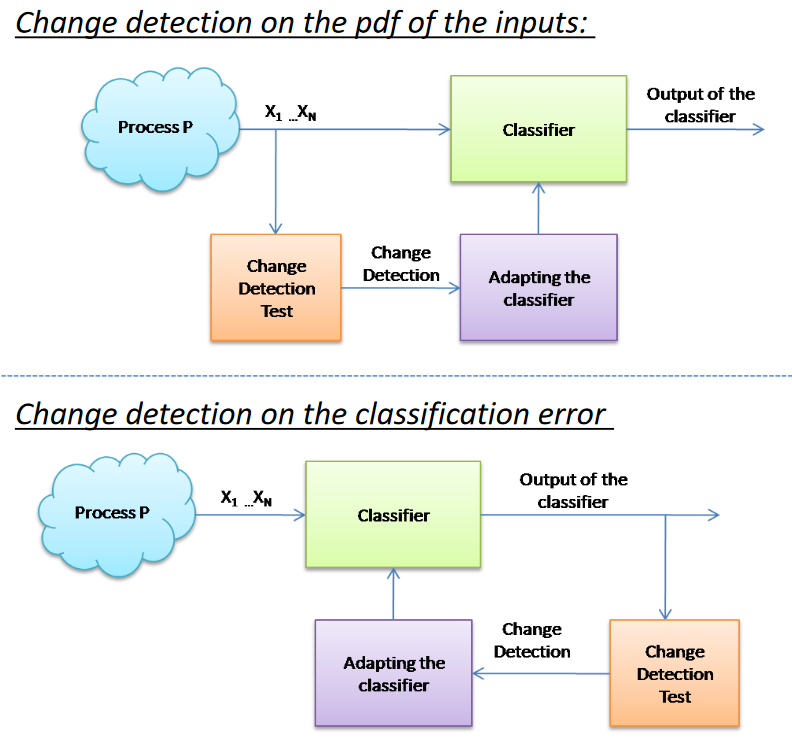
\includegraphics[scale=0.35]{../Images/ActivePDFAcc.png}
        \centering
        \caption{Monitoring schemes}
      \end{figure}
      For both monitoring schemes we still have to detect if a change has happened and when. In any case we can't directly analyze the data, so we must extract some features that are $iid$.

      To make the process easier to understand we can define three main steps:
      \begin{itemize}
        \item \emph{Concept drift detection}: Where ad-hoc triggers designed to detect changes by inspecting sequences of data or derived features are employed. A non-exausting list of method is provided below:
        \begin{itemize}
          \item Data-based methods
          \begin{itemize}
            \item Limit checking: where we test if a given (measured) variable exceeds (indicating a change) or not a known absolute limit. This method is easy to implement however the choice of the threshold is a critical issue which can lead to high/low sensitivity to change.
            \item Binary threshold
          \end{itemize}
          \item Statistical-based methods
          \begin{itemize}
            \item Statistical Hypothesis tests
            \item Change-Point Methods
            \item Change detection tests
            \begin{itemize}
              \item CUMSUM tests
              \item Shiryaev-Robert test
              \item CI-CUSUM test, NPCUSUM test
              \item ICI-based change detection test
              \item Semiparametric log-likelihood criterion (SPLL)
            \end{itemize}
          \end{itemize}
        \end{itemize}

        These methods not only provide detection of the change, but also an estimation of the time instant the process becomes non-stationary. In this way by knowing the time at which the change is detected $\hat{T}$ and the estimate of the time of change $T_{ref}$ we can estimate the real time of change $T^{*}$ as shown in the figure below.
        \begin{figure}[H]
          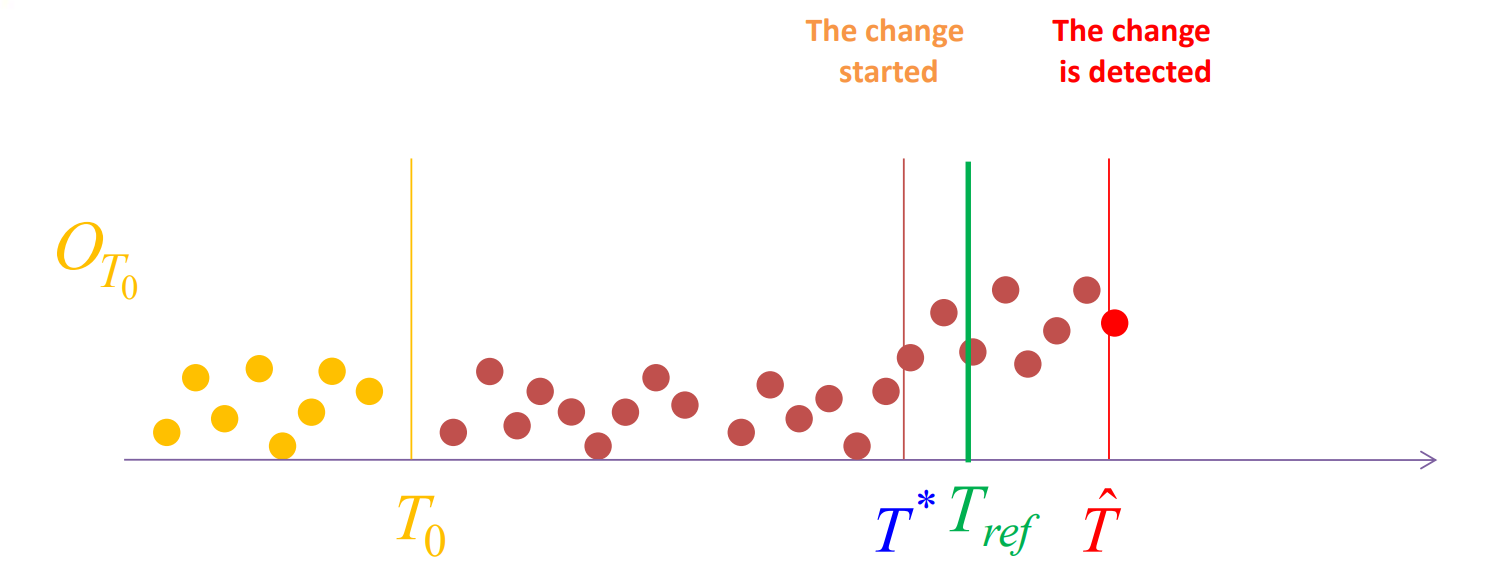
\includegraphics[scale=0.35]{../Images/ChangeDetectionTime.png}
          \centering
          \caption{Change detection time estimate}
        \end{figure}
        \item \emph{Identification of the new state}: Additionally we want to know, based on some features, if the current state (or concept) is recurring (has already happened). This should help with ciclo-stationary processes which can have different properties based on the interval of observation. 
        \begin{figure}[H]
          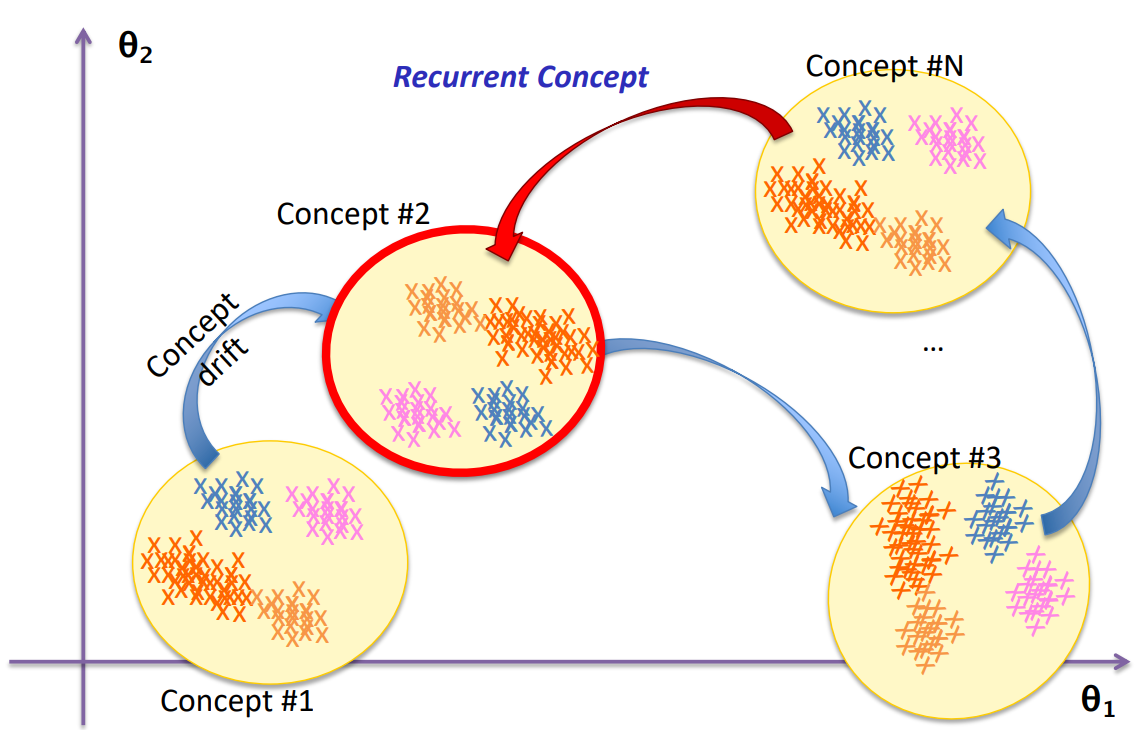
\includegraphics[scale=0.35]{../Images/RecurringCOnceptsScenario.png}
          \centering
          \caption{Recurring concepts' scenario}
        \end{figure}
        \item \emph{Retrain the application}: Covered in the previous section.
      \end{itemize}

      In general, we can make some relevant remarks:
      \begin{itemize}
        \item Being acquainted with learning techniques is a plus in everybody’s background.
        \item Most of the time we can assume that the process generating the data is time invariant. When it is not, we need to pay attention.
        \item Learning in a changing environment must be considered and represents a key property intelligent systems should possess.
      \end{itemize}

  \section{Deep Learning for IoT}
    In this section we want to explore how to start from the single IoT unit and get an ecosystem perspective. In general Deep-Learning for IoT concerns three macro topics such as:
    \subsection{On-Device Learning}
      While in the previous section we already discussed learning in the presence of concept drift, now we need to port everything on the device. In the IoT context the drift can be caused by:
      \begin{itemize}
        \item Changes in the environment
        \item Changes in the user's behavior/interest
        \item Faults/malfunctioning affecting the hardware or sensors/actuators
        \item Aging effects or thermal drifts affecting the sensors
      \end{itemize}
      In general perturbed, incorrect and missing data can hence heavily affect the subsequent processing phase to possibly induce wrong decisions or on-the-field reactions. 

      To address this issue both active and passive solutions can be employed as long as instance selection is the updating method since instance weighting and multiple models are not feasible on device.

      A current challenge in the field concerns back propagation, since all the activations and errors must be stored to update the network. A proposed solution is to walk away from conventional CNN and move to trainless clustering algorithms like $kNN$ (k Nearest Neighbors). In this solution a general feature extractor
      extracts features from the input and after the N-Dimensional feature space has been reduced we can use some previously stored features to run the clustering algorithms. An objection may be raised since this in not much different from decoupling the last part of a CNN, however it's difficult to identify at which layer
      we can extract the most significant features.

      While clustering algorithms can solve some of our issues they impose significant memory demand and computational complexity.
      \begin{figure}[H]
        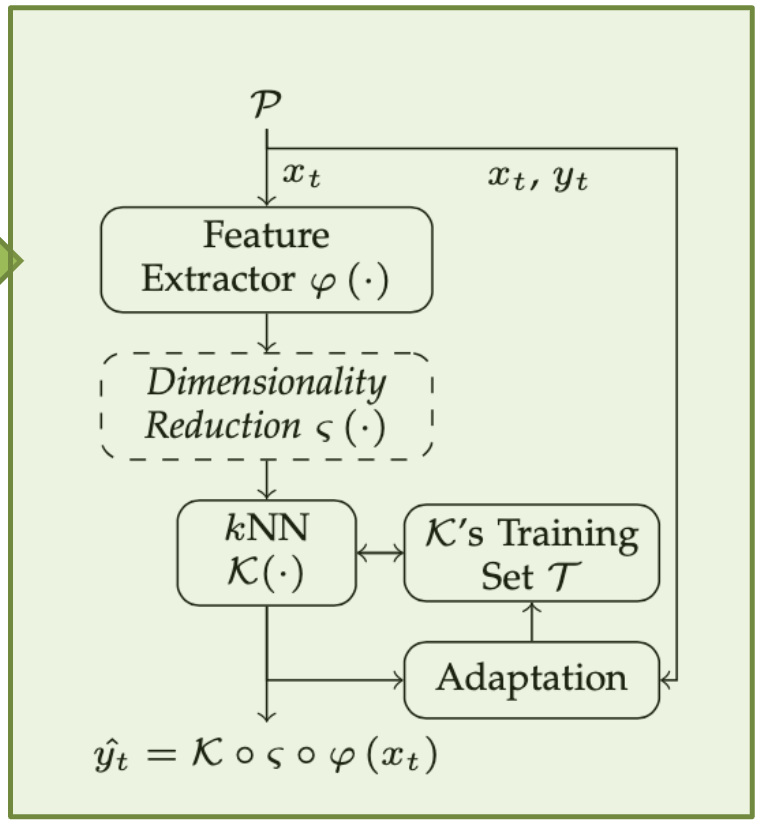
\includegraphics[scale=0.35]{../Images/kNNArch.png}
        \centering
        \caption{kNN Hybrid Architecture}
      \end{figure}

      Moreover, the knowledge base of the kNN is a feature space (Which is always smaller than the sample space), and can be further condensed by identifying the smallest subset of training data that can correctly classify all the training samples.

      The adaptation mechanism can be:
      \begin{itemize}
        \item \textbf{Passive}: The adaptation is carried out at each new supervised Sample.
        \item \textbf{Active}: The adaptation is triggered by a CUSUM-based change-detection mechanism.
        \item \textbf{Hybrid}: Where the hybrid update continuously adapts the knowledge base ($T$) over time thanks to the passive adaptation while the active adaptation present in the hybrid
        update can quickly discard obsolete knowledge when a change is detected and set a bound on the memory footprint of the knowledge base.
      \end{itemize}

      \begin{figure}[H]
        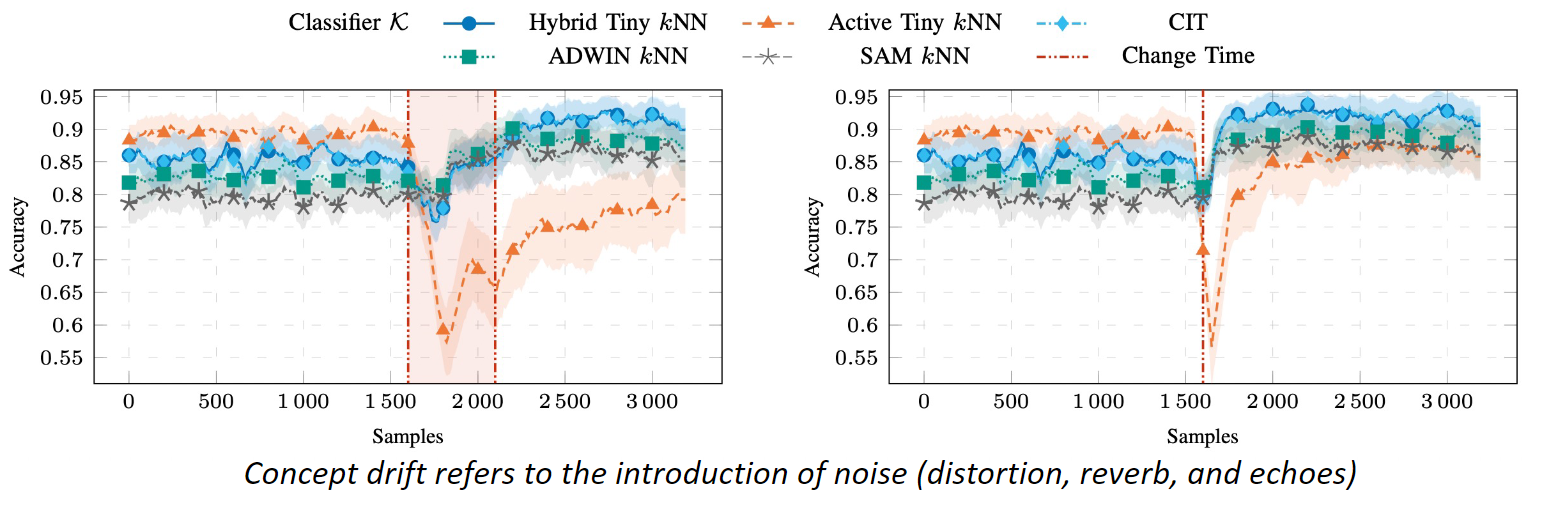
\includegraphics[scale=0.35]{../Images/HybridPerformance.png}
        \centering
        \caption{kNN Hybrid Architecture Performance}
      \end{figure}

      This topic is still actively discussed in the research space in particular regarding \emph{Semi-Supervised TinyML} to remove the need for labels in the training and classification process and \emph{Automatic design, development and deployment for On-line Tiny Machine Learning}
    \subsection{Distributed CNNs}
      While until now we have explored how to reduce the size of CNNs to fit our tiny devices another approach may be useful when IoT is involved. In particular, we want to exploit the ability of an IoT node to communication with its neighbors by assigning each devide a single layer of Network. In this way each node in the system (which can include different platforms) can execute the layer and
      transmit the results to next node. Now the problem is how to identify the optimal allocation of CNN layers on a set of heterogeneous IoT units since on a single network we can run multiple models independently (figure on the left) or share some resources if the models have common layers (figure on the right).

      \begin{figure}[H]
        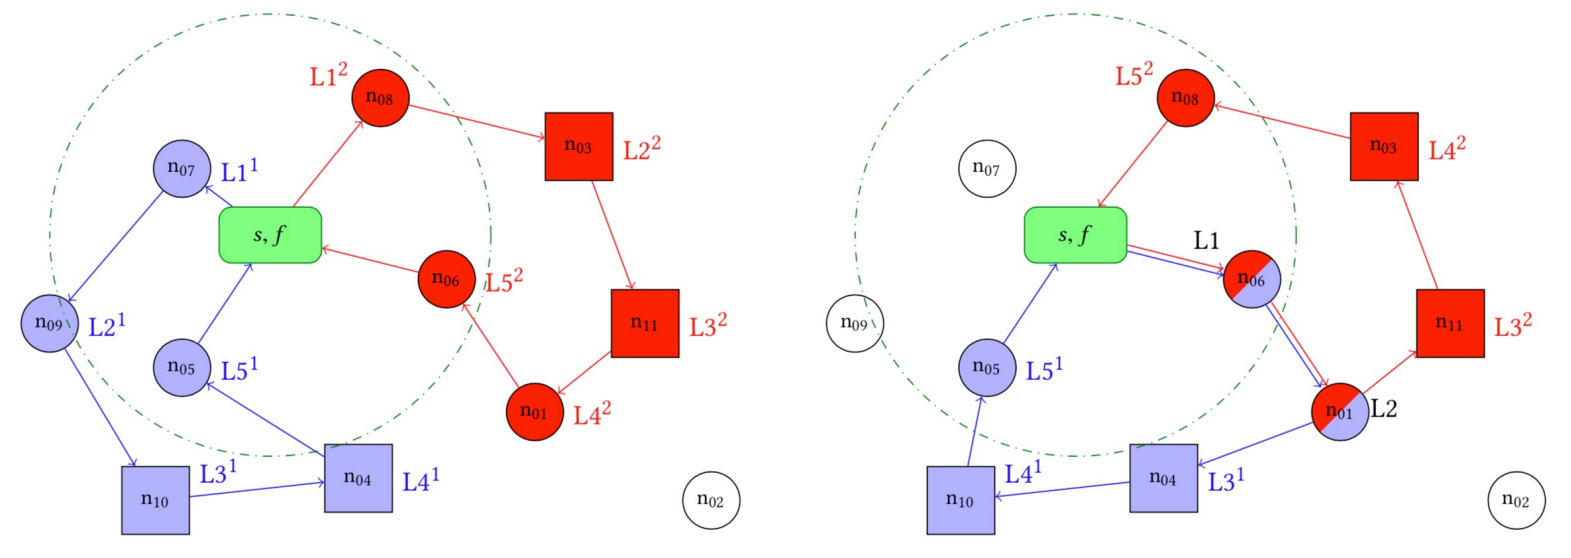
\includegraphics[scale=0.35]{../Images/DistributedCNN.png}
        \centering
        \caption{Examples of Distributed CNNs (Different colors indicate different models)}
      \end{figure}

      With this framework the possibilities are endless, however we should keep in mind the transmission overhead both in terms of power and latency.
    \subsection{Federated Learning}
    Federated learning is a decentralized machine learning approach that enables collaborative model training while preserving data privacy. It addresses the challenges associated with centralizing data from multiple sources by allowing individual participants to train a shared model using their local data. The process involves iterative rounds of communication between a central server and distributed devices, such as smartphones or edge devices, where the data resides.
    
    In federated learning, during each communication round, the central server sends the current model parameters to the participating devices. The devices then perform local model updates using their respective data while keeping the data itself locally stored and secure. The locally updated models are then aggregated by the central server, either by averaging or other aggregation methods, to generate a new global model. This process ensures that the server gains insights from the combined knowledge of the distributed devices without accessing their raw data.
    
    The key advantages of federated learning lie in its privacy-preserving nature and its ability to accommodate data distributed across various devices. By keeping data local, federated learning reduces privacy risks associated with data transmission and storage by employing Homomorphic Encryption, Secure
    Multi-Party Computation and Differential Privacy (keep in mind that is still possible to extract the training data from the model). Additionally, it overcomes challenges related to data silos and enables model training on edge devices with limited connectivity. This decentralized approach allows for broader participation, as data owners can contribute to the model training process while retaining control over their sensitive information.
    
    This approach is particularly useful in scenarios where we deal with:
    \begin{itemize}
      \item Pervasively Distributed devices (smartphones, IoT devices).
      \item Privacy Issues, Sensitive Data (personal, medical, banking data).
      \item User-needs require cooperation (data and computational power).
      \item System Heterogeneity (devices can be different in HW characteristics).
      \item Statistical Heterogeneity (possible non-independent and identically distributed (non-IID) data across the set of devices).
      \item Non-Stationary Environment (seasonality effects, changes in users’ behavior).
    \end{itemize}

    Various architectures have been formulated based on the fact that devices may have different data and feature spaces:
    \begin{itemize}
      \item Horizontal: Local datasets share the same feature space, but they are different in samples.
      \item Vertical: The sample space of the local data sets is the same (or similar) but the feature space is different. The clients are trained with the same data, using different features.
      \item Federated Transfer Learning: Local datasets differ both in samples and features.
    \end{itemize}

    \begin{figure}[H]
      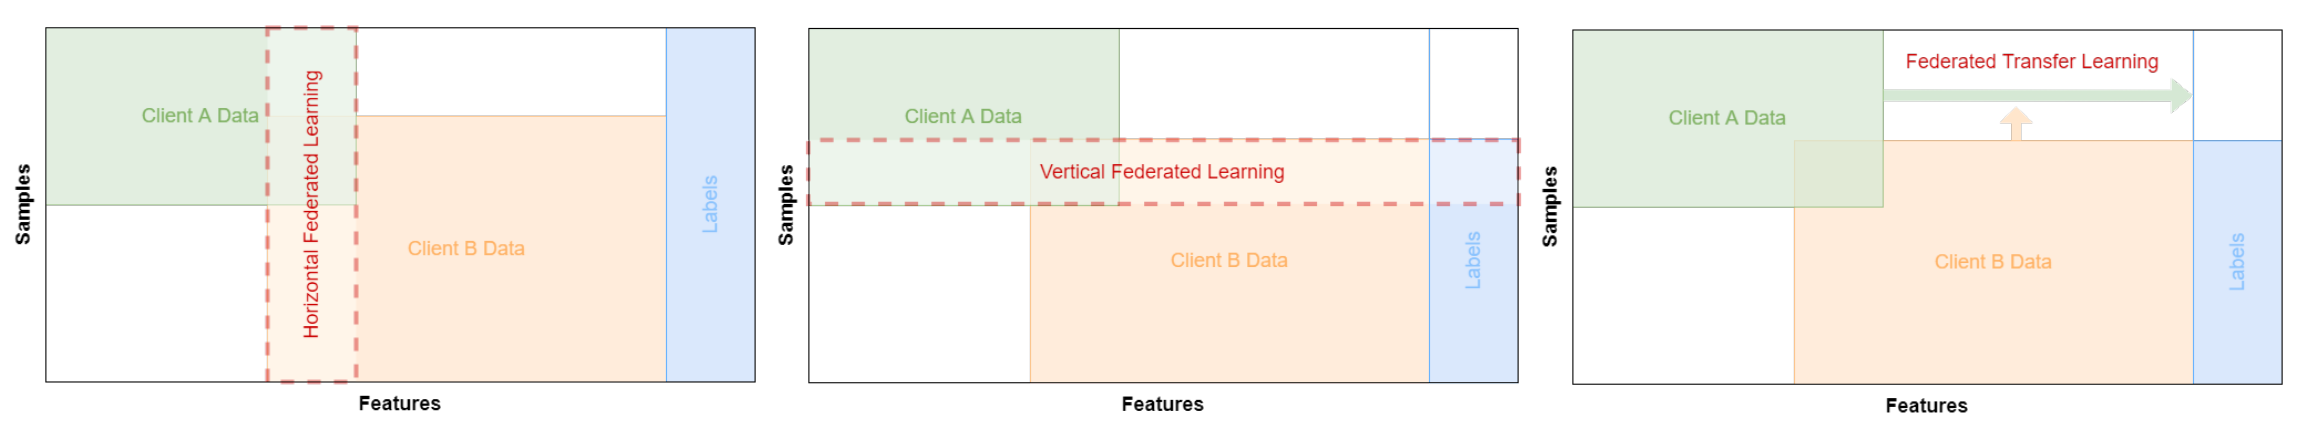
\includegraphics[scale=0.2]{../Images/FLArch.png}
      \centering
      \caption{Federated learning architectures}
    \end{figure}

    For completion, we list the most popular aggregation mechanism for federate learning named \emph{Federated Average (FedAVG)} which is an iterative process consisting in:
    \begin{itemize}
      \item 1. Server sends initialized model’s
      parameters to the clients
      \item 2. Clients perform their local updates
      \item 3. Clients send back their updated
      parameters
      \item 4. Server aggregates the parameters
      (simple average)
      \item 5. Then, the parameters are updated
      and sent to the clients
      \item 6. Go back to point 2
    \end{itemize}
    
\newpage
\begin{thebibliography}{9}

  \bibitem{SNet}
  Forrest N. Iandola and Song Han and Matthew W. Moskewicz and Khalid Ashraf and William J. Dally and Kurt Keutzer,
  \textit{SqueezeNet: AlexNet-level accuracy with 50x fewer parameters and $<$0.5 MB model size},
  2016.

  \bibitem{MNet}
  Andrew G. Howard and Menglong Zhu and Bo Chen and Dmitry Kalenichenko and Weijun Wang and Tobias Weyand and Marco Andreetto and Hartwig Adam  
  \textit{MobileNets: Efficient Convolutional Neural Networks for Mobile Vision Applications},
  2017.

  \bibitem{ENet}
  Mingxing Tan and Quoc V. Le
  \textit{EfficientNet: Rethinking Model Scaling for Convolutional Neural Networks},
  2019.
  
  \end{thebibliography}




  \end{document}